%; whizzy paragraph
%; whizzy-paragraph "^\\\\dancersection"
% -initex iniptex -latex platex -format platex -bibtex jbibtex -fmt fmt
% 以上 whizzytex を使用する場合の設定。

%     Tokyo Debian Meeting resources
%     Kansai Debian Meeting resources
%     Copyright (C) 2008 Junichi Uekawa
%     Copyright (C) 2008 Nobuhiro Iwamatsu

%     This program is free software; you can redistribute it and/or modify
%     it under the terms of the GNU General Public License as published by
%     the Free Software Foundation; either version 2 of the License, or
%     (at your option) any later version.

%     This program is distributed in the hope that it will be useful,
%     but WITHOUT ANY WARRANTY; without even the implied warranty of
%     MERCHANTABILITY or FITNESS FOR A PARTICULAR PURPOSE.  See the
%     GNU General Public License for more details.

%     You should have received a copy of the GNU General Public License
%     along with this program; if not, write to the Free Software
%     Foundation, Inc., 51 Franklin St, Fifth Floor, Boston, MA  02110-1301 USA

%   Pdf作成手順
% dvipdfmx debianmeetingresume2011-fuyu.dvi
%  preview (shell-command (concat "evince " (replace-regexp-in-string "tex$" "pdf"(buffer-file-name)) "&"))
% 画像ファイルを処理するためにはebbを利用してboundingboxを作成。
%(shell-command "cd image2012-fuyu; ebb *.png")


% progress memo:
% 2019/12 kansai-2020/11がマージ対象
% イベント等でない場合は理由を書くこと。
% 必要な変更点は FIXME で記録しています。

%%ここからヘッダ開始。

\documentclass[mingoth,a4paper]{jsarticle}
\usepackage{monthlyreport}
\usepackage[dvips]{xy} % for advi workaround. Bug #452044
\usepackage{ulem}
\usepackage{wrapfig}
%\usepackage{pygmentize}

% コードハイライトの為の設定 for 201706 tokyo
\makeatletter\chardef\pdf@shellescape=\@ne\makeatother
\usepackage{minted}

% ページ調整のため部分的に2段組に
\usepackage{multicol}

\begin{document}

\begin{titlepage}
\thispagestyle{empty}

\hspace*{-2.5cm}

\includegraphics{../2012/image2012-natsu/gudeb.eps}\\
\\
\\
\rotatebox{10}{\fontsize{32}{32} {\gt 東京エリア/関西Debian勉強会}}

%\vspace*{-1.5cm}
\hspace*{11cm}
\includegraphics[height=6cm]{../2005/image200502/openlogo-nd.eps}\\
\vspace*{0.1cm}
\hfill あんどきゅめんてっど でびあん 2021年冬号 2021年12月31日 初版発行
\end{titlepage}

\newpage
\thispagestyle{empty}\mbox{}
\newpage

% section の代わりの環境 -- 改訂する。
\renewcommand{\dancersection}[2]{%
\newpage
あんどきゅめんてっど でびあん 2021年冬号
%
% top line
\vspace{0.1mm}\\
{\color{dancerlightblue}\rule{\hsize}{2mm}}

%
% middle text
%
\begin{minipage}[t]{0.6\hsize}
\color{dancerdarkblue}
\vspace{1cm}
\section{#1}
\hfill{}#2\\
\end{minipage}
\begin{minipage}[t]{0.4\hsize}
\vspace{-2cm}
\hfill{}
\includegraphics[height=8cm]{image200502/openlogo-nd.eps}\\
\vspace{-5cm}
\end{minipage}
%
%
{\color{dancerdarkblue}\rule{0.74\hsize}{2mm}}
%
\vspace{2cm}
}

\setcounter{page}{1}
\begin{minipage}[]{0.2\hsize}
 \definecolor{titleback}{gray}{0.9}
 \colorbox{dancerlightblue}{\rotatebox{90}{\fontsize{80}{80}
{\gt \color{dancerdarkblue}デビアン勉強会} }}
\end{minipage}
\begin{minipage}[]{0.8\hsize}
\hrule
\vspace{1mm}
\hrule
\setcounter{tocdepth}{1}
{\small
 \tableofcontents}
\vspace{1mm}
\hrule
\vspace{3cm}

\end{minipage}

% FIXME: 本文を追加すること。
%-------------------------------------------------------------------------------
\dancersection{Introduction}{DebianJP}
%-------------------------------------------------------------------------------

\subsection{東京エリアDebian勉強会}

 Debian勉強会へようこそ。これからDebianの世界にあしを踏み入れると
 いう方も、すでにどっぷりとつかっているという方も、月に一回Debianについ
 て語りませんか?

 Debian勉強会の目的は下記です。

\begin{itemize}
 \item \underline{Debian Developer} (開発者)の育成。
 \item 日本語での ``\underline{開発に関する情報}'' を整理してまとめ、アップデートする。
 \item \underline{場}の提供。
 \begin{itemize}
  \item 普段ばらばらな場所にいる人々が face-to-face で出会える場を提供
    する。
  \item Debian のためになることを語る場を提供する。
  \item Debianについて語る場を提供する。
 \end{itemize}
\end{itemize}

 Debianの勉強会ということで究極的には参加者全員がDebian Packageをがりがり
 と作るスーパーハッカーになった姿を妄想しています。情報の共有・活用を通し
 て Debianの今後の能動的な展開への土台として、 ``場'' としての空間を提供す
 るのが目的です。

\subsection{関西 Debian 勉強会}

 関西 Debian 勉強会はDebian GNU/Linux のさまざ
 まなトピック(新しいパッケージ、Debian 特有の機能の仕組、Debian 界隈で起
 こった出来事、などなど)について話し合う会です。

 目的として次の三つを考えています。
 \begin{itemize}
  \item MLや掲示板ではなく、直接顔を合わせる事での情報交換の促進
  \item 定期的に集まれる場所
  \item 資料の作成
 \end{itemize}

 それでは、楽しい一時をお楽しみ下さい。
 
%収録予定
%202010
%-------------------------------------------------------------------------------
\dancersection{DebianでのRust}{上川純一}
%-------------------------------------------------------------------------------

Rust\cite{rustsite}というプログラミング言語をご存知ですか?私はC++よりメモリ管理
などが便利になっていてコンパイルさえ通ると大体メモリの所有権についての問題が解決
しているということで勉強してみることにしました。

執筆時点ではVersion 1.47.0が公開されており、比較的安定しているようです。

良い解説書\cite{rustbook}がオンラインにあり、日本語にも活発に翻訳\cite{rustjp}さ
れているようです。

しかしどうもDebianにはFirefoxのビルドに必要だからパッケージされているだけのよう
な気がしなくもない。

\subsection{DebianユーザとしてRustプログラムを書いてみる}

まず入門書を読み始めるとおもむろにRustのサイトからバイナリパッケージをインストー
ルするためにシェルスクリプトをウェブからダウンロードしてきて実行するように書いて
あります。

\begin{commandline}
$ curl --proto '=https' --tlsv1.2 https://sh.rustup.rs -sSf | sh
\end{commandline}
%$ -- for emacs

しかしインストールの副作用は何があるのかとかを確認したいし、アンインストールする
ときに何をしたら良いのかなど考えるのが面倒ですよね。そこでDebianユーザとしてはパッ
ケージを利用したい。Debianのパッケージを利用するにはどうしたらよいかを解説します。

\begin{commandline}
$ sudo apt install cargo rustc 
\end{commandline}
%$ -- for emacs

まずBusterでは最初にリリースされたときは1.33\footnote{2019年2月28日にリ
リース}だったのですが2020年9月に比較的新しい1.41.1\footnote{2020年2
月27日にリリースされているようです
\url{https://blog.rust-lang.org/2020/02/27/Rust-1.41.1.html}}にアップデー
トされました。firefox-esr のセキュリティーアップデートの依存関係だったよ
うです。The Rust Book\cite{rustbook}が1.41.0を前提としているのでまぁこれ
でいいんじゃないでしょうか。

\subsubsection{エディタの設定}

Emacsを使っているのならelpa-rust-modeを入れておきましょう。

\begin{commandline}
$ sudo apt install elpa-rust-mode  # for local emacs.
\end{commandline}
%$ -- for emacs


Vim は\url{https://github.com/rust-lang/rust.vim#installation}にたくさん
書いてあるのですがちょっとよくわかってません。

\subsubsection{シンプルなプログラムを書く}

チュートリアルに従ってプログラムを書いてみます。

\begin{commandline}
fn main() {
   println!("Hello, world!");
}
\end{commandline}

コンパイルして実行してみます。

\begin{commandline}
$ rustc helloworld.rs 
$ ./helloworld
Hello, world! 
\end{commandline}

\subsubsection{Cargoを使う}

Rustcを直接つかうよりはCargoというビルド管理ツールを使うことが多いようで
す。テンプレートの生成からビルドやテストの実行までやってくれます。Crate
とよばれるRustのパッケージシステムが利用できるようになります。

Cargo関連のファイルはホームディレクトリ以下の\verb!~/.cargo/! に作成され
ます。

cargo newでプロジェクトのテンプレートが作成され、Hello world とだけ出力
するsrc/main.rsが生成されます。cargo buildでビルド。cargo runで実行、
cargo testでテストが実行されます。

\begin{commandline}
$ cargo new 名前
$ cd 名前
$ cargo build
$ cargo run
Hello, world!
$ cargo clean
\end{commandline}
%$ -- for emacs

Cargo.tomlというファイルに依存関係を記述することができます。このCrateパッ
ケージインストールはDebianの管理下ではなくユーザのホームディレクトリ以下
にインストールされます。

\subsection{Docker で使うには}

Dockerイメージで使うということもあるでしょう。公式で提供されているDocker
イメージがあるのでそれを使うのが手っ取り早いと思われます。Debianのパッケー
ジを使いたい場合はパッケージをインストールすればよいです。

\begin{commandline}
FROM debian

RUN apt-get clean && apt-get update && apt-get install -yq \
      make \
      rustc \
      && apt-get clean
\end{commandline}

しかしながらDockerhubにはすでに公式のDockerイメージが提供されており、
rustパッケージはDebian BusterにRustupでRustの最新版をインストールしたも
のになっています\cite{docker:rust}。パッケージとして提供されていないのは
気になりますがDockerイメージの中なのでアンインストールの方法などを考える
必要がなく、影響範囲が限定されており、便利に使えそうです。

\begin{commandline}
FROM rust 
\end{commandline}


\subsection{Debian Developer としてのRustパッケージ}

Rustパッケージをメンテンスしているチーム\cite{rust:debianwiki}がいるので
Wikiページなどに情報がまとまっています。Crateのパッケージングについての
資料\cite{debcargo-conf}に解説があります。

パッケージのためのツールとしてdebcargoというものを使うようです。

\begin{commandline}
$ apt update && apt install debcargo
\end{commandline}
%$ -- for emacs

おそらく一番の困難は、RustのCrateは複数のバージョンが共存できるように作
られているのですが、Debian側のポリシーとしては単一のバージョンのライブラ
リをできるだけ使いたいです。そうすると古いバージョンを要求される場合はそ
れをできるだけ新しいバージョンで置き換えることになるでしょう。大量にパッ
チを書くことになりそうです。

debcargo の動作原理ですが、Cargoの利用するcargo.tomlファイル
\cite{cargo-toml}に依存関係の情報があるのでそれを利用してDebianパッケー
ジを生成するようです。

\begin{thebibliography}{1}
 \bibitem{rustbook} \url{https://doc.rust-lang.org/book/}
 \bibitem{rustsite} \url{https://www.rust-lang.org/}
 \bibitem{rustjp} ``Rustの日本語ドキュメント/Japanese Docs for Rust''
	 \url{https://doc.rust-jp.rs/}
 \bibitem{rust:debianwiki} \url{https://wiki.debian.org/Teams/RustPackaging}
 \bibitem{debcargo-conf} ``Packaging a crate for Debian''
	\url{https://salsa.debian.org/rust-team/debcargo-conf/blob/master/README.rst}
 \bibitem{cargo-toml} ``The Manifest Format''
	\url{https://doc.rust-lang.org/cargo/reference/manifest.html}
 \bibitem{docker:rust} ``Rust -- Docker Official Images'' \url{https://hub.docker.com/_/rust} 
\end{thebibliography}

%202011
%-------------------------------------------------------------------------------
\dancersection{DebianでのPython}{杉本典充}
%-------------------------------------------------------------------------------

\subsection{はじめに}

Debian では多くのプログラム言語の実行環境、ライブラリ及びアプリケーションのパッケージを多数提供しています。今回はPythonについてDebianではどのようにパッケージをメンテナンスしているのかを調べてみました。

\subsection{Pythonについて}

Python とは Debian などの linux 環境のみならず他の OS でも実行することが可能な
マルチプラットフォームのプログラミング言語の1つです。
2015年に機械学習のプラットフォームである tensorflow がオープンソース化され、 tensorflow には Python のライブラリが豊富なことから Python の人気が上がってきています。

Pythonのwebサイト(\url{https://www.python.org/}) では
初心者向けのチュートリアル\footnote{\url{https://www.python.org/about/gettingstarted/}}、
Pythonの言語仕様やクラス・関数の仕様書\footnote{\url{https://docs.python.org/3/}}などの多くの情報を公開しています。特に開発者向けの情報ではPEP(Python Enhancement Proposals)\footnote{\url{https://www.python.org/dev/peps/}}と呼ばれるPythonを
よりよくするための提案の募集を公開しており\footnote{DebianにもDEPという似たような仕組みがあります。\url{https://dep-team.pages.debian.net/}}、コーディング規約やライブラリの廃止勧告、互換性の説明など多岐にわたる情報を公開しています。


\subsection{DebianにおけるPython情報の取り扱いについて}

\subsubsection{基本な情報}

Debian における Python 関連の情報は以下ページにまとまっています。

\begin{itemize}
\item Python - Debian Wiki \url{https://wiki.debian.org/Python/}
\item Debian Python Policy \url{https://www.debian.org/doc/packaging-manuals/python-policy/}
\end{itemize}

Debian Project では、Python の実行環境をメンテナンスするチーム(cpython-team)とライブラリ及びアプリケーションをメンテナンスするチーム(Debian Python Team)の2つに分かれて活動しています。2つのチームの主な違いを表\ref{tb:pythonteam}に示します。

\begin{table}[htb]
  \begin{center}
  \caption{Debian ProjectにおけるPythonのチーム情報}
  \begin{tabular}{|c|c|c|} \hline
    チーム名 & cpython-team & Debian Python Team(DPT) \\ \hline
    役割 & 実行環境のメンテナンス & ライブラリとアプリケーションのメンテナンス \\ \hline
    メーリングリスト & debian-python@lists.debian.org & (同左) \\ \hline
    IRC & \#debian-python & (同左) \\ \hline
    wiki & - & \url{https://wiki.debian.org/Teams/PythonTeam} \\ \hline
    gitリポジトリ & \url{https://salsa.debian.org/cpython-team} & \url{https://salsa.debian.org/python-team} \\ \hline
  \end{tabular}
  \label{tb:pythonteam}
  \end{center}
\end{table}

「Debian Python Policy」\footnote{\url{https://www.debian.org/doc/packaging-manuals/python-policy/}} を読んでみて、パッケージの話で大事そうなところを以下に挙げてみます。

\begin{itemize}
\item python3 へ移行しましょう
\item python のインタプリタのディレクトリ配置やファイル名の規則(例:/usr/bin/python3、/usr/bin/python3.8)
\item python ライブラリのパスの規則(debian パッケージでは /usr/lib/python\{3,2.7\}/dist-packages/ 配下に配置する)
\item python のライブラリやアプリケーションの debian パッケージ名の命名規則(python3 系用であれば python3-* の形式とすること、モジュール名にアンダースコアが入っている場合は debian パッケージ名ではハイフンに置換すること)
\item pythonプログラムについて
  \begin{itemize}
  \item シェバンには \#!/usr/bin/env interpreter\_name は使わないこと
  \item \#!/usr/bin/python3 または \#!/usr/bin/python3.y としてdebianが提供するデフォルトのバージョンを指定すること
  \end{itemize}
\item python の debian パッケージ化を支援するための debhelper の拡張として dh-python パッケージがある
\end{itemize}


\subsubsection{cpython-teamについて}

cpython-team チームの \url{https://salsa.debian.org/groups/cpython-team/-/group_members} に表示されるメンバーは Matthias Klose(@doko) さん1名のみです。

Klose さんが メンテナンスしている \url{https://tracker.debian.org/pkg/python3.9} を確認してみると、maintainer にはチームでなく Klose さんの名前が書いてあります。そのため 1 人でメンテナンスしているようです。

2020 年 11 月 時点の unstable においては python-2.7、3.8、3.9 のパッケージを提供しており、現在は python-3.9 のデバッグ作業を行っています\footnote{\url{https://bugs.debian.org/cgi-bin/pkgreport.cgi?tag=python3.9;users=debian-python@lists.debian.org}}。


\subsubsection{Debian Python Team(DPT)について}

Debian Python Team(DPT)のメンバーは \url{https://wiki.debian.org/Teams/PythonTeam} に記載があり、2020 年 11 月現在では 20 名でメンテナンスしているようです。チームでメンテナンスしているパッケージの一覧は次のURLで見ることができます。

\begin{itemize}
\item \url{https://qa.debian.org/developer.php?email=team%2Bpython%40tracker.debian.org}
\end{itemize}  


Debian Python Team(DPT)に参加するには チームのポリシードキュメントを読み、応諾した上で参加することを求めています。チームのポリシーを記載したドキュメントは以下のページにあります。

\begin{itemize}
\item \url{https://salsa.debian.org/python-team/tools/python-modules/blob/master/policy.rst}
\end{itemize}  

このページに記載しているポリシーにはおおよそ以下の内容が書かれています。

\begin{itemize}
\item チームへ参加方法
  \begin{itemize}
  \item 以下3つを書いたメールを debian-python@lists.debian.org へ送信する
    \begin{itemize}
    \item なぜ参加したいのか
    \item \url{https://salsa.debian.org} にログインするアカウント名
    \item ポリシードキュメント(policy.rst)を読み、受諾することの宣言
    \end{itemize}
  \end{itemize}
\item パッケージメンテナンスについて
  \begin{itemize}
  \item debian パッケージ内の debian/control ファイルの Maintainer フィールド及び Uploaders フィールドの意味
  \item git-buildpackage を使ったパッケージメンテナンスの説明
  \end{itemize}
\end{itemize}

また、Python のパッケージを作るにあたっては debian/control、debian/rules などのファイルの書き方の説明が以下のページ記載されています。

\begin{itemize}
\item \url{https://wiki.debian.org/Python/LibraryStyleGuide}
\item \url{https://wiki.debian.org/Python/AppStyleGuide}
\end{itemize}


\subsubsection{pypiパッケージをdebianパッケージに変換する}

プログラム言語にはそれぞれライブラリやアプリケーションをパッケージ化して配布するサイトを持っていることが多いです。そして Debian ではそれぞれのプログラム言語のライブラリを debian パッケージへ変換する debian パッケージを配布しており、以下のページに情報があります。

\begin{itemize}
\item \url{https://wiki.debian.org/AutomaticPackagingTools}
\end{itemize}
    
Python におけるライブラリやアプリケーションの配布サイトは \url{https://pypi.org/} が有名です。上記 URL で紹介している Python 向けの debian パッケージへの変換ツールは「python3-stdeb」 パッケージに入っている「py2dsc-deb」コマンドがよさそうに思いました\footnote{pypi2debパッケージは依存パッケージがとても多くperl関連のパッケージが大量にインストールされます。}。

試しに py2dsc-deb コマンドを使って pypi が配布するパッケージを debian パッケージに変換してみました。debian/compatバージョンは "9" として変換しているようです。

\begin{commandline}
$ sudo apt-get install python3-stdeb python-all dh-python
$ wget https://files.pythonhosted.org/packages/53/20/4019a739b2eefe9282d3822ef6a225250af964b117356971bd55e274193c/
ws4py-0.5.1.tar.gz
$ py2dsc-deb ws4py-0.5.1.tar.gz
$ ls -l deb_dist
l合計 128
-rw-r--r-- 1 norimitu norimitu 38224 11月 19 13:58 python3-ws4py_0.5.1-1_all.deb
drwxr-xr-x 8 norimitu norimitu  4096 11月 19 13:58 ws4py-0.5.1
-rw-r--r-- 1 norimitu norimitu   916 11月 19 13:58 ws4py_0.5.1-1.debian.tar.xz
-rw-r--r-- 1 norimitu norimitu   869 11月 19 13:58 ws4py_0.5.1-1.dsc
-rw-r--r-- 1 norimitu norimitu  5480 11月 19 13:58 ws4py_0.5.1-1_amd64.buildinfo
-rw-r--r-- 1 norimitu norimitu  1024 11月 19 13:58 ws4py_0.5.1-1_amd64.changes
-rw-r--r-- 1 norimitu norimitu  5419 11月 19 13:58 ws4py_0.5.1-1_source.buildinfo
-rw-r--r-- 1 norimitu norimitu  1377 11月 19 13:58 ws4py_0.5.1-1_source.changes
-rw-r--r-- 2 norimitu norimitu 51408  2月 26  2020 ws4py_0.5.1.orig.tar.gz

$ cat deb_dist/ws4py-0.5.1/debian/compat
9
\end{commandline}

また、python のパッケージをインストールするコマンド "pip" でインストールしたときに binding ライブラリのコンパイルも一緒に行うライブラリ "mysqlclient" を試してみると、以下のコマンドで debian パッケージに変換できました。

\begin{commandline}
$ sudo apt-get install python3-stdeb python3-all-dev dh-python libmysqlclient-dev
$ wget https://files.pythonhosted.org/packages/a5/e1/e5f2b231c05dc51d9d87fa5066f90d1405345c54b14b0b11a1c859020f21/
mysqlclient-2.0.1.tar.gz
$ py2dsc-deb mysqlclient-2.0.1.tar.gz
$ ls -l deb_dist
合計 264
drwxr-xr-x 11 norimitu norimitu  4096 11月 19 14:15 mysqlclient-2.0.1
-rw-r--r--  1 norimitu norimitu  1236 11月 19 14:15 mysqlclient_2.0.1-1.debian.tar.xz
-rw-r--r--  1 norimitu norimitu   927 11月 19 14:15 mysqlclient_2.0.1-1.dsc
-rw-r--r--  1 norimitu norimitu  6192 11月 19 14:15 mysqlclient_2.0.1-1_amd64.buildinfo
-rw-r--r--  1 norimitu norimitu  1394 11月 19 14:15 mysqlclient_2.0.1-1_amd64.changes
-rw-r--r--  1 norimitu norimitu  5795 11月 19 14:15 mysqlclient_2.0.1-1_source.buildinfo
-rw-r--r--  1 norimitu norimitu  1464 11月 19 14:15 mysqlclient_2.0.1-1_source.changes
-rw-r--r--  2 norimitu norimitu 87807  7月  3 03:55 mysqlclient_2.0.1.orig.tar.gz
-rw-r--r--  1 norimitu norimitu 90744 11月 19 14:15 python3-mysqlclient-dbgsym_2.0.1-1_amd64.deb
-rw-r--r--  1 norimitu norimitu 48584 11月 19 14:15 python3-mysqlclient_2.0.1-1_amd64.deb

$ cat deb_dist/mysqlclient-2.0.1/debian/compat
9
\end{commandline}


\subsection{終わりに}

debian における Python パッケージをどういうチームがどのようにパッケージを作成、メンテナンスしているか調べてみました。皆さんも Python や他のプログラム言語のライブラリやアプリケーションを debian パッケージ化し、debian ライフをお楽しみください。

\subsection{参考情報}

\begin{itemize}
\item \url{https://wiki.debian.org/Python/}
\item \url{https://www.debian.org/doc/packaging-manuals/python-policy/}
\item \url{https://salsa.debian.org/python-team/tools/python-modules/blob/master/policy.rst} 
\item \url{https://wiki.debian.org/Python/LibraryStyleGuide}
\item \url{https://wiki.debian.org/Python/AppStyleGuide}
\end{itemize}

%202008kansai
\dancersection{Makefile から CMake に高速で入門する}{Yosuke OTSUKI}

\subsection{はじめに}

CMake はkitware 社によるマルチプラットフォームで使用できるビルドツールです。
Unix 系の OS で使用されている gmake, ninja などを始め、Windows の nmake や Visual Studio の solution ファイルも出力できます。
また、unit test と .rpm や .deb 形式 \footnote{debian 公式のパッケージの規格は満たしていません。あくまでも野良パッケージです。} の作成もできます。

Go や Rust など最近のコンパイルが必要な言語は、言語独自のビルド・パッケージ機構を持っているものが多く CMake は必要ないと思います。
しかし、C/C++, Fortran など古くてコンパイルが必要な言語には便利です。
cmake は明文化されていない仕様が多く、熟練した技術者でも意外な使い方でハマることがあると思います。そこで本書では Makefile と CMakeLists.txt  を比較して cmake の習得時間を短くしようと思います。繰り返しになりますが、以下が狙いです。

\subsection{本著の狙い}
\begin{itemize}
  \item{Makefile が書ける人が、CMakeLists.txt を書けるようになる手助けをする}
  \item{CMake の明文化されてない仕様を説明して、はまらないようにする}
\end{itemize}

また、本著は CUI による cmake の使用を前提としています。IDE との連携は説明しません。\footnote{著者が cmake と IDE の連携に詳しくないのは秘密です。}
サンプルはすべて、C 言語をビルドすることにします。
ただし、パッケージングについては CMakeLists.txt のみの説明しています。
なお、本著では執筆時時点の debian buster の環境で動作確認をしています。
cmake のバージョンは 3.13.4-1 です。

note: footnote に記載しているリンクは 2020/08/21  日時の時点ではアクセスを確認しています。
\clearpage

%==============================================================================
\subsection{最初に単一ソースコードのビルド}
%==============================================================================
最初にサンプルでは C 言語のコードを単体ビルドすることにします。
そのコードをビルドする Makefile を示したあとに、同じことを CMakeLists.txt で記述した例を示します。

\vspace{1em}
C 言語のコード
\begin{commandline}
#include <stdio.h>

int main(){
    printf("Hello World\n");
    return 0;
}
\end{commandline}
\vspace{1em}
Makefile
\begin{commandline}
all: main.c
	gcc -o hello_world $?
\end{commandline}
\vspace{1em}
CMakeLists.txt
\begin{commandline}
# 必要となる最小の cmake のバージョンを指定
cmake_minimum_required(VERSION 3.13 FATAL_ERROR)

# プロジェクト名 executable の名前になる
project(hello_world)

# 文字列を標準出力に出力する。変数 CMAKE_C_COMPILER は c コンパラの絶対パス。
# cmake 実行後に生成される CMakeCache.txt の中に変数は記述される。
message ("*** ${CMAKE_C_COMPILER}")

# executable のビルド
add_executable(hello_world main.c)

# インストールのディレクトリ構成を GNU の構成にする (bin/, lib/ ...)
include(GNUInstallDirs)

# executable のみなので、bin のディレクトリをインストール対象にする
install(TARGETS hello_world DESTINATION ${CMAKE_INSTALL_BINDIR})
\end{commandline}

cmake の syntax を説明をします。
cmake\_minimum\_required は必須です。ただし、FATAL\_ERROR は省くことができます。
project で対象となる executable の名前を決めています。
add\_executable でプロジェクトのソースコードを指定し、ビルドします。
include(GNUInstallDirs) で GNU のディレクトリ構造でインストールするようにしています。
他の方法も使うことができますが、パッケージング時に絶対パスとなってしまうのでこの方法がおすすめです。

CMakeLists.txt には autools の dist clean に相当するコマンドが存在しません。
そのため、作業用のディレクトリを作りその中で cmake を呼び出します。(ここでは build という作業用のディレクトリを作ります)
そうすることで、ソースコードのディレクトリに一時的なファイルを作らなくて良くなります。
\footnote{cmake だけの用語かもしれませんが out of source build と呼ばれる方法です。}
ただし、OSS プロジェクトの中にはソースコードでビルドの実行を要求するものもあります。
以下のコマンドを実行して、autools の configure に相当することをします。

\vspace{1em}
実行コマンド
\begin{commandline}
mkdir build
cd build

# autools の configure に相当。-G で出力するビルドシステムを指定 (省略可能)
cmake -G "Unix Makefiles" -DCMAKE_INSTALL_PREFIX=`pwd`/build ../

make
make install
cd ..
\end{commandline}
正常終了すると 00.hello\_world/hello\_world が生成されます。

-G はcmake generator option です。省略するとデフォルトの Makefile が生成されます。
使用できる generator については、cmake -G で確認してください。
使用している OS によって異なります。\footnote{https://cmake.org/cmake/help/v3.18/manual/cmake-generators.7.html}

build/CMakeCache.txt を調べてみましょう。
ビルドに使用する linker, archiver や インストール先のディレクトリなどが記載されています。
中には、デフォルトで値が決まっているものもあります。
ここでは、autools の \-\-prefix に相当する CMAKE\_INSTALL\_PREFIX を使って cmake の変数の上書きについて説明します。
CMAKE\_INSTALL\_PREFIX はデフォルトでは /usr/local が値としてされています。
cmake では基本的には変数の上書きは推奨されていません。 \footnote{set(CMAKE\_INSTALL\_PREFIX /home/yosukesan PATH FORCE "") などで強制的な上書きは可能です。}
その代わりに、cmake の起動時に -D\{変数名\} として変数の初期値を与える方法が一般的です。

%==============================================================================
\subsection{外部ライブラリのリンク}
%==============================================================================

次に外部のライブラリとリンクをしてみましょう
説明のために、共有ライブラリと静的ライブラリを直接リンクします。
その後、一般的なプロジェクトで利用される共有・静的リンクどちらでも使用できる方法を紹介します。
以下の C 言語のコードのように pthread を使いたい場合を例とします。

\vspace{1em}
C 言語
\begin{commandline}
#include <pthread.h>
#include <stdio.h>

void *work(void* parg){
    int *val = (int*)parg;
    printf("worker tid=%d\n", *val);
    *val = 100;
}

int main (){
    pthread_t handle; 
    int data = 0;

    pthread_create(&handle, NULL, work, &data);    
    pthread_join(handle, NULL);
    printf("final = %d\n", data);

    return 0;
}
\end{commandline}

例えば、Makefile で共有ライブラリをリンクする場合、以下のように書きます。

\vspace{1em}
Makefile
\begin{commandline}
shared: main.c
	gcc $? -lpthread
static: main.c
	gcc $? /usr/lib/x86_64-linux-gnu/libpthread.a
\end{commandline}

\subsubsection{共有ライブラリ}

では、cmake でビルドする例を見ていきましょう。
共有ライブラリのリンクは比較的簡単に行なえます。

\vspace{1em}
CMakeLists.txt
\begin{commandline}
cmake_minimum_required(VERSION 3.13 FATAL_ERROR)

project(pthread_task)
add_executable(pthread_task main.c)

# プロジェクトとリンクするライブラリ名を指定すれば良い。システムライブラリならば、自動的に見つけてくれる。
# なお、先頭の lib は自動的に保管されるので付けてはいけない。 (libpthread.so)
target_link_libraries(pthread_task pthread)

include(GNUInstallDirs)
install(TARGETS pthread_task DESTINATION ${CMAKE_INSTALL_BINDIR})
\end{commandline}

新しく、target\_link\_library() というコマンドを使いました。
使い方については、スクリプト中のコメントを参照してください。
pthread に拡張子 (.so か .a) を付けない場合、共有ライブラリがリンクされます
cmake の実行は先の例と同じです。

\subsubsection{静的ライブラリ}

次に、静的なリンクをする方法を説明します。
共有ライブラリと異なる方法を使用します。\footnote{試した限り、共有ライブラリと同じ方法でもビルドはできました。しかし、Seg ります。これにどハマリしました。}

\vspace{1em}
CMakeLists.txt
\begin{commandline}
cmake_minimum_required(VERSION 3.13 FATAL_ERROR)

project(pthread_task)
add_executable(pthread_task main.c)

# cmake のライブラリ用のプロジェクトに外部ライブラリをインポートする。
add_library(libpthread STATIC IMPORTED)

# ライブラリの path を指定
set_target_properties(libpthread PROPERTIES IMPORTED_LOCATION /usr/lib/x86_64-linux-gnu/libpthread.a)

# ヘッダーの path を指定
set_target_properties(libpthread PROPERTIES INTERFACE_INCLUDE_DIRECTORIES /usr/include)

target_link_libraries(pthread_task libpthread)
include (GNUInstallDirs)
install(TARGETS pthread_task DESTINATION ${CMAKE_INSTALL_BINDIRS})
\end{commandline}

add\_library というコマンドを追加しました。
静的なライブラリをリンクする場合は、一度 cmake のライブラリのオブジェクトにインポートする必要が有ります。

\subsubsection{推奨する方法 find\_package()}

今までの方法では、ライブラリの絶対パスを明示的に指定してきました。
しかし、ビルドに必要な複数のライブラリの絶対パスを、全て記述するのは効率的ではありません。
また、テスト時などはインストール先を、システムパスではない PATH にするかもしれません。

そのような場合、find\_package() というコマンドを使用します。\footnote{\url{https://discourse.cmake.org/t/how-to-statically-link-external-library-by-target-link-libraries/1718}}
特定のパッケージについて、検索用の cmake スクリプトを書いておくと、find\_package() を呼び出すだけで、指定されたルートディレクトリから自動的に lib と include のパスを検索してくれます。

\vspace{1em}
CMakeLists.txt
\begin{commandline}
cmake_minimum_required(VERSION 3.13)
project(pthread_task)

# thread の中で pthread が使いたいのでフラグを立てる
set(THREADS_PREFER_PTHREAD_FLAG TRUE)

# thread ライブラリを検索。findThread.cmake が提供されているので使えるコマンド
find_package(Threads REQUIRED)

add_executable(pthread_task main.c)

# thread ライブラリをリンク
target_link_libraries(pthread_task PRIVATE Threads::Threads)

include(GNUInstallDirs)
install(TARGETS pthread_task DESTINATION ${CMAKE_INSTALL_BINDIR})
\end{commandline}

pthread のような一般的なものは、検索用のスクリプトが cmake に備わっています。\footnote{\url{https://cmake.org/cmake/help/latest/module/FindThreads.html}}
しかし、特定の用途でしか使わないライブラリの場合、例えば gmp などは自分で検索用のスクリプトを準備する必要があります。\footnote{\url{https://github.com/shohirose/cmake-find-package/blob/master/FindGMP.cmake}}
FLOSS が cmake をビルドシステムとしている場合、多くの場合検索用のスクリプトも提供される場合が多いです。
例えば、kitware 社の VTK ライブラリでは、ソースコードとともに findVTK.cmake というスクリプトが提供されています。

%==============================================================================
\subsection{分割コンパイルとリンク}
%==============================================================================

この例では、自分で作成したライブラリと自分の executable にリンクします。
この例でも共有と静的なリンクの方法を説明します。
分割コンパイルは、外部ライブラリのリンクほど難しくはありません。

整数の変数を入力引数とし、1 を加算して返す簡単な関数を自作しました。

\vspace{1em}
my\_inc.h
\begin{commandline}
#pragma once

extern int inc(int val);
\end{commandline}

\vspace{1em}
my\_inc.c
\begin{commandline}
#include <stdio.h>
#include "my_inc.h"

int inc(int val){
    printf("%d\n", ++val);
}
\end{commandline}

\vspace{1em}
main.c
\begin{commandline}
#include "my_inc.h"

int main(){
    int val = 0;
    inc(val);
    return 0;
}
\end{commandline}

\vspace{1em}
Makefile
\begin{commandline}
CFLAGS=-W -Wall
CC=gcc

.PHONY: libmyinc

all: libmyinc
	gcc $(CFLAGS) main.c libmyinc.so

libmyinc: my_inc.c
	gcc $(CFLAGS) -shared -o libmyinc.so -fPIC $?

clean:
	rm *.o *.so *.out
\end{commandline}
上記の Makefile に対応する CMakeLists.txt は以下です。
\vspace{1em}
CMakeLists.txt
\begin{commandline}
cmake_minimum_required(VERSION 3.13 FATAL_ERROR)
project(sample)

# 共有ライブラリをビルドする
add_library(my_inc SHARED my_inc.c)

add_executable(sample main.c)
target_link_libraries(sample my_inc)

include(GNUInstallDirs)
install(TARGETS my_inc DESTINATION ${CMAKE_INSTALL_LIBDIR})
install(TARGETS sample DESTINATION ${CMAKE_INSTALL_BINDIR})
install(TARGETS my_inc.h DESTINATION ${CMAKE_INSTALL_INCLUDEDIR})
\end{commandline}

動的なリンクでも、静的なリンクでもcmake の実行は先の例と同じです。
add\_library() というコマンドを追加しました。共有ライブラリを作成する場合は SHARED、STATIC と記述すると静的ライブラリが生成されます。何も記述しない場合は、共有ライブラリが生成されます。

\clearpage

%==============================================================================
\subsection{ctest で単体テスト}
%==============================================================================

自作のライブラリと自作のアプリのビルドができるようになったので、単体テストを組み込みます。
先程の、my\_inc() コマンドをテストする test() というコマンドを書いた test.c というソールコードを追加しました。このソースコードをビルドして単体テストを実行しましょう。

\vspace{1em}
test.c
\begin{commandline}
#include <stdbool.h>
#include <assert.h>

#include "my_inc.c"

bool test ()
{
    assert(inc(0) == 1);
    assert(inc(65535) == 65536);

    return true;
}

int main(){
    return test() ? 0 : -1;
}
\end{commandline}

\vspace{1em}
Makefile
\begin{commandline}
CFLAGS=-W -Wall
CC=gcc
ld_lib_path=

.PHONY: libmyinc

all: libmyinc
	gcc $(CFLAGS) main.c libmyinc.so

libmyinc: my_inc.c
	gcc $(CFLAGS) -shared -o libmyinc.so -fPIC $?

test:
	gcc $(CFLAGS) -o test.out test.c libmyinc.so
	echo -e "#!/bin/bash -x\nexport LD_LIBARY_PATH=`pwd`\n./test.out"

clean:
	rm *.o *.so *.out *.sh
\end{commandline}

\vspace{1em}
MakeLists.txt
\begin{commandline}
cmake_minimum_required(VERSION 3.13 FATAL_ERROR) 
project(sample)
add_library(my_inc my_inc.c)
add_executable(sample main.c)
target_link_libraries(sample my_inc)

enable_testing()
add_executable(test_sample test.c)
target_link_libraries(test_sample my_inc)
message ("${PROJECT_SOURCE_DIR}")
add_test(NAME unit_test COMMAND $<TARGET_FILE:test_sample> WORKING_DIRECTORY ${PROJECT_SOURCE_DIR}/build)

include(GNUInstallDirs)
install(TARGETS sample DESTINATION ${CMAKE_INSTALL_BINDIR})
install(TARGETS my_inc DESTINATION ${CMAKE_INSTALL_LIBDIR})
install(FILES my_inc.h DESTINATION ${CMAKE_INSTALL_INCLUDEDIR})

\end{commandline}

enable\_testing() と add\_test() というコマンドを追加しました。
テストを実行するために、CMAKE\_BUILD\_TYPE という変数を実行時に指定して、初期化をしています。
これは ctest を実行する場合、デフォルトの BUILD\_TYPE が実行対象に含まれないためです。 

\begin{commandline}
mkdir build
cd build
cmake -DCMAKE_INSTALL_PREFIX=`pwd`/../  -DCMAKE_BUILD_TYPE=Release ../
make

# --stop-on-failure テストに失敗したところで停止
# --verbose 詳細なメッセージを出す。実行したテストの絶対パスを表示してほしいので使っている
ctest --stop-on-failure --verbose
make install
cd ..
\end{commandline}

ctest コマンドでテストを実行します。 
引数なしでも実行は可能ですが、おすすめはサンプルの通りです。

%==============================================================================
\subsection{パッケージング}
%==============================================================================

今まで説明してきたものをすべて追加して、lib の作成、executable の作成をした後に単体テストを行い、パッケージングをするスクリプトが以下です。
CMake は正式な Debian の基準に沿った .deb は生成できません。
しかし、複数の形式のパッケージングに対応しているので社内ツールなど、それほど品質が必要ないものには便利かもしれません。

\begin{commandline}
cmake_minimum_required(VERSION 3.13 FATAL_ERROR)

project(sample)
add_library(my_inc SHARED my_inc.c)
add_executable(sample main.c)
target_link_libraries(sample my_inc)

enable_testing()
add_executable(test_sample test.c)
target_link_libraries(test_sample my_inc)
message ("${PROJECT_SOURCE_DIR}")
add_test(NAME unit_test COMMAND $<TARGET_FILE:test_sample> WORKING_DIRECTORY ${PROJECT_SOURCE_DIR}/build)

include(GNUInstallDirs)
install(TARGETS sample DESTINATION ${CMAKE_INSTALL_BINDIR})
install(TARGETS my_inc DESTINATION ${CMAKE_INSTALL_LIBDIR})
install(FILES my_inc.h DESTINATION ${CMAKE_INSTALL_INCLUDEDIR})

# prerequisite apt-get install build-essetial rpm
# .deb と .rpm をパッケージングする
set (CPACK_GENERATOR "DEB" "RPM")
set (CPACK_DEBIAN_PACKAGE_MAINTAINER "yosukesan")
set (CPACK_PACKAGE_VERSION_MAJOR "0")
set (CPACK_PACKAGE_VERSION_MINOR "1")
include (CPack)
\end{commandline}

上記の例では、.deb と .rpm を作成します。
cmake は debuild と rpmbuild を呼び出して実行するので、もしインストールしていない場合はコメント行の apt を実行してください。

上記のスクリプトを実行する場合は、以下で実行してください。
cpack でパッケージングを行っています。
今回は .deb と .rpm のみですが FreeBSD, Qt, MacOS, Windows (Wix) などにも対応しています\footnote{\url{https://cmake.org/cmake/help/v3.13/manual/cpack-generators.7.html}}。

\begin{commandline}
mkdir build
cd build
cmake -DCMAKE_INSTALL_PREFIX=`pwd`/../  -DCMAKE_BUILD_TYPE=Release ../
make
ctest
cpack
cd ..
\end{commandline}

先に説明しましたが include (GNUInstallDirs) を指定して CMAKE\_INSTALL\_\{BINDIR, LIBDIR, INCLUDEDIR\} をインストール先にしています。
このようにしないと、インストール先が絶対パスとして格納されたパッケージが出来上がってしまいます。

\subsection{まとめ}

Makefile と CMakeLists.txt を対比しつつ説明してきました。
Windows のネイティブ環境にも対応しているので、複数の OS に対してバイナリーを出力しなければならないときなどには便利です。

最後に私は以下ぐらいしか記憶していません。下記のキーワードで検索して、コマンドの仕様や、関連する仕様について cmake のドキュメントを読んだり、使用例を探したりしています。
\begin{itemize}
  \item{add\_executable() : executable のビルド}
  \item{add\_library() : ライブラリのビルド}
  \item{target\_link\_library() : executable とライブラリのリンク}
  \item{install() : make install をやるためのコマンド}
  \item{ctest, enable\_testing() and add\_test() : 単体テストに必要}
  \item{cpack : パッケージングのコマンド}
\end{itemize}

\subsection{参考文献}

\begin{itemize}
\item \url{http://opencv.jp/cmake/cmake_tutorial.html} (accessed 2020/Aug/20th)
\item \url{https://www.qoosky.io/techs/814fda555d} (accessed 2020/Aug/20th)
\item \url{https://blog.usejournal.com/creating-debian-packages-cmake-e519a0186e87?gi=1efc3589ce87} (accessed 2020/aug/20th)
\end{itemize}

\vspace{\fill}
本資料は GPL v 2.0 のライセンスで公開いたします。

%202007
\dancersection{10年ぶりのニューラルネットワーク}{野首貴嗣}

過去、2010年3月に行われた第62回東京エリアDebian勉強会では
「ニューラルネットワークで画像認識してみた」
というタイトルで本庄弘典さんが発表をされていました。

それから10年が経過した2020年7月(勉強会開催)現在、ニューラルネットワークをとりまく
状況がどのように変化したかを俯瞰的に見ていきます。

また、個人的に開発、公開している成果についても紹介します。

\subsection{ニューラルネットワークのお気持ち}

まず、ニューラルネットワークについての厳密ではない、なんとなくなお気持ちで
概要を解説します。

パーセプトロン(\url{https://ja.wikipedia.org/wiki/%E3%83%91%E3%83%BC%E3%82%BB%E3%83%97%E3%83%88%E3%83%AD%E3%83%B3})と呼ばれる、人間の脳(ニューロン)を模した演算ユニットがあります。
これは入力信号Xに対し、重みWを乗じバイアスbを加算した結果Yをえる単純なユニットです。さらに、Yに対し活性化関数と呼ばれる関数を適用しその結果を分類タスクの結果として考えます。

分類が正しいなら1を、間違っているなら0を返す関数と考え、実際に用意したデータをもちいて訓練を行います。訓練は、逆誤差伝播(バックプロパゲーション)という手法を使い、求められた結果と訓練データ上の正解との誤差を最小化するよう、重みを調整していきます。

単一のパーセプトロンはANDやORを表現することができます。パーセプトロンの式は線形分離境界を表していると考えることで直感的に理解できるでしょう。
さらには、XORは実現できないことも理解できると思います(1つの直線で分離できないため)。

ニューロンを増やしたり、多段に接続することで、より複雑な非線形分離が可能となります。この段数が概ね4段以上になったものをディープラーニングと呼ぶことが多いようです。

\subsection{ブレイクスルー}

2012年に、Googleが''Using large-scale brain simulations for machine learning and A.I.''(\url{https://blog.google/topics/machine-learning/using-large-scale-brain-simulations-for/})というblog記事と論文
(\url{http://static.googleusercontent.com/media/research.google.com/ja//archive/unsupervised_icml2012.pdf})
を公開しました。
16コアをもつマシン169台を駆使し、大量の画像を訓練することで教師なしで人体や猫の特徴を獲得したと話題になりました。このときに採用されたアーキテクチャはAutoAEncoderと呼ばれるものです。

AutoEncoderは入力側と出力側が等しくなるように構成された多段ニューラルネットワークで、入出力画像よりも小さなベクトル表現によって、入力画像の特徴を獲得することができるものです。
AutoEncoderが行っていることは、一種の次元圧縮ともいえます。ニューラルネットワークを用いない次元圧縮手法もありますが、多段ニューラルネットワーク(ディープラーニング)が実用になることを示した大きな一歩でした。

\subsection{ブレイクスルー実現要素}

従来のニューラルネットワークが抱えていた課題を解決した要素にはさまざまなものがあります。

\begin{description}
\item[計算資源の向上] \mbox{} \\
  私がニューラルネットワークに触れた1995年の時点で、実際に利用されていたコンピュータのスペックは次のようなものでした。
  \begin{itemize}
  \item PA-RISC 25Mhz
  \item メモリ16MB
  \end{itemize}
  そもそも利用可能なメモリが少なく、大きなニューラルネットワーク構造を持つこと自体が困難でした。現代においてはスマートフォンでも4GB程度のメモリを搭載するものも珍しくありません。
\item[GPGPUの一般化] \mbox{} \\
  CPU自体も当時と比較してかなり高速にはなりましたが、単一コアあたりの処理能力向上には限界が見えつつあります。一方でグラフィックス処理向けに設計されたGPUをより一般的なコンピューティングに応用する環境が整備されてきました。\\
  GPUは特に並列計算を得意としており、多段ニューラルネットワークの演算とは非常に相性がよく、その方向へ進化していっています。
\item[大規模データセットの拡充]  \mbox{} \\
  Googleの猫の例で活躍したのは、Google photosやFacebook album等、画像データを大量に収集できるプラットフォームの存在でした。\\
  さらに、ラベル(物体の種別情報)を付与したデータセットも増えていきます。これにはクラウドソーシングサービスの拡充(Amazon Mechanical Turk, Cloudworks等)も寄与しています。
\item[技術的な進歩]  \mbox{} \\
  多段ニューラルネットワークが抱えていた他の問題として、勾配消失/発散問題がありました。逆誤差伝播をする際に、層が増えることによって伝播すべき誤差がどんどん小さくなってしまったり、逆に大きくなったりする問題です。\\
  要因の一つに、活性化関数があります。シグモイド関数を使うことが昔は一般的でしたが、この関数が取りうる値は0〜1しかありません。より幅広い値を扱える活性化関数(ReLU等のランプ関数)の出現により、より大きな勾配を扱えるようになりました。\\
  また勾配のクリッピングによって、勾配爆発を抑えることができるようになりました。
  その他Batch Normalizationなどの正規化手法も学習の安定化に寄与しています。
\item[分散表現の活用]  \mbox{} \\
  単語や抽象的なカテゴリーといったものを表現するために分散表現(埋め込み表現)が活用できることがわかり、自然言語処理などへの活用が広がりました。word2vecは単語埋め込み表現の最たる活用例です。
\item[データ拡張]  \mbox{} \\
  既存のデータを変形したり、ノイズをのせるなどのデータ拡張技術が主に画像認識分野で発達しています。これにより、学習データを水増しすることができ、認識制度向上に寄与しています。
\item[教師データを必要としない学習]  \mbox{} \\
  一般的な教師あり学習には正解データを用意する必要があり、その作成にはコストがかかります。一方でword2vecのような、教師データを必要としない手法が発達してきています。\\
  既存のデータの一部をマスクしたり、並べ替えたりして正解を予想させることで、対象となるデータの特徴をうまく表現する情報を獲得することができます(表現学習)。
\item[敵対的生成ネットワーク]  \mbox{} \\
  生成モデルと識別モデルを組み合わせ、互いを競わせるように学習させることで、現実には存在しない画像などを生成する手法が提案され、広く使われています。
\end{description}

\subsection{環境}

\begin{description}
\item[データサイエンティストブーム] \mbox{} \\
  2000年代よりデータサイエンティストブームが発生し、ゼロ年代は統計的手法が広まりました。
  その流れは2010年台でも継続し、深層学習手法にも波及しています。
  数多くのMOOCsプラットフォームも立ち上がり、安価で良質な学習環境が整備されています。
\item[コンペティションの隆盛] \mbox{} \\
  Kaggle, SIGNATEといったコンペティションサイトが立ち上がり、技術者の研鑽が日々なされています。
\item[実行環境の充実] \mbox{} \\
  かねてから GPGPU 環境は AWS, GCE などで提供されていましたが、それ以外にも無料でGPUの利用が可能なGoogle Colaboratoryといったサービスが使えるようになり、ブラウザさえあれば環境構築不要で機械学習が行えるようになりました。
\end{description}

\subsection{もたらされた変化}

\begin{description}
\item[人を越える精度/能力] \mbox{} \\
  画像認識分野では、ImageNet(\url{http://image-net.org/})というデータセットでいかに高い認識精度を達成するか、という試みが行われています。2012年にディープラーニングベースの手法 AlexNet が登場して以来、急速にその精度は向上し、2015年には ResNet によって人間の認識能力を超える精度を達成しました(参考: \url{https://www.slideshare.net/ren4yu/ss-234439652/21})。\\
  自然言語の分野でも、Stanford Question Answering Dataset (SQuAD) (\url{https://rajpurkar.github.io/SQuAD-explorer/})などで人間の正答率を超える正答率を達成しています。\\
  問題を分類タスクに落とし込むことができ、十分な学習データを用意することができれば、機械学習モデルは人間を超える精度を達成できる可能性を示しています。
\item[生成モデル] \mbox{} \\
  たくさんの画像やテキストデータ、音楽データから、新しいデータを生成するモデルが広く使われるようになりました。\\
  主に敵対的生成ネットワークによる成果ですが、テキストに関しては言語モデルベースの手法(GPT-2等)が主流です。\\
  さらにこれらを応用することで、画像復元(inpainting)や自動着色、さらには描画支援(GauGAN)といったことが実現できています。
\item[機械翻訳] \mbox{} \\
  ディープラーニング以前の機械翻訳は統計ベースの手法が利用されていました。この手法はあまり流暢ではない文が生成されがちという欠点があったのですが、ニューラル機械翻訳によって、その問題は大きく改善されました。\\
  一方でGPUが持つメモリがボトルネックとなり、語彙を多くもたせることが難しくなりました。そのため、単語より小さな単位(サブワード)でトークンを区切ることによって語彙を抑える手法が主流となってきています。\\
  ニューラルネットワークの学習は多くがend-to-endで行えるため、正確な単語区切りや品詞を考慮しなくても良くなったという事情もあります。\\
  その副作用として、多言語を一度に扱えるようにもなりました。サブワードより小さい、バイト単位で区切る手法もあります。この場合、デコード時に正しいバイト列であることを保証する必要性があります。
\end{description}

\subsection{新たな課題}

ニューラルネットワーク固有の課題も登場しています。

\begin{description}
\item[翻訳ミス] \mbox{} \\
  統計ベースの機械翻訳でも翻訳ミスはありましたが、ニューラル機械翻訳の場合、それを見つけることが難しくなっています。なまじ流暢な結果を出力してしまうため、注意深く見ないと訳抜けなどを見逃してしまいがちです。
  また、統計ベースでは、原文と翻訳文のフレーズ対応が処理の関係上あきらかだったのですが、ニューラル機械翻訳ではend-to-endな学習になったことで、翻訳文と原文との対応づけが明らかでなくなったというデメリットもあります。\\
  他に、逆の意味を出力してしまうことがある問題もあります。これも訳文の対応付けが不明瞭なため、原因をさぐることは難しい問題です。\\
  同じ文言を繰り返し生成するという、ニューラル機械翻訳特有の問題もあります(参考事例: \url{https://www.slideshare.net/ToshiakiNakazawa/nlp2017-nmt-tutorial/79})。
\item[データセットとバイアス] \mbox{} \\
  近年よく問題としてとりあげられるものに、バイアスがあります。これは、学習に使ったデータセット内に偏りがあった場合、特に注意をしないとそれがそのまま機械学習モデルに反映されてしまいます。\\
  たとえば、多くの場合英語で''sister''という単語は姉・妹の区別をつけることはあまりなく、機械翻訳でそれを日本語にした際に、文脈に応じて出現しやすい方に訳してしまうことが発生します。
\item[敵対的サンプル] \mbox{} \\
  人間が見るとパンダなのに、識別モデルにはテナガザルに見えるような画像が有名です(参考: \url{https://speakerdeck.com/settenqb/ji-jie-xue-xi-tosekiyuritei?slide=5})。このように機械翻訳モデルを騙す画像を生成する技術と、それを防衛する技術が互いにしのぎを削っています。
\item[バックドア] \mbox{} \\
  訓練に用いるデータセットに悪意あるデータを混ぜることで、バックドアを仕掛けるという手法もあります。クラウドソーシングなどを使う際には、用途によってはそのような問題があることを想定しておく必要もあるでしょう。
\end{description}

\subsection{フレームワーク}

よく使わていた(いる)代表的なフレームワークには以下のものがあります。

\begin{itemize}
\item 古参
  \begin{itemize}
  \item Torch7
  \item Caffe
  \item Theano
  \end{itemize}
\item 現代的なもの
  \begin{itemize}
  \item Chainer
  \item PyTorch
  \item TensorFlow
  \item Keras
  \item Darknet
  \end{itemize}
\end{itemize}

どれも多次元配列を扱うことができ、自動微分機能を備えています。

\subsection{Web/JavaScriptランタイム}

先に述べたようなフレームワークで訓練されたモデルを、ブラウザやJavaScriptで実行するフレームワークがいくつかあります。

\begin{itemize}
\item WebDNN
  \begin{itemize}
  \item https://mil-tokyo.github.io/webdnn/ja/
  \item 日本発
  \item 複数のフレームワークに対応
  \item 現在開発はinactive
  \end{itemize}
\item TensorFlow.js
  \begin{itemize}
  \item https://www.tensorflow.org/js
  \item TensorFlow公式
  \item 訓練もサポート
  \item 多くの訓練済みモデルを配布
  \item https://github.com/tensorflow/tfjs-models
  \end{itemize}
\item ONNX.js
  \begin{itemize}
  \item https://github.com/microsoft/onnxjs
  \item フレームワーク共通フォーマットONNXに対応
  \item 対応している演算に制限あり
  \end{itemize}
\end{itemize}

\subsection{作成したものの紹介}

WebDNNを用いて、いくつかのデモサイトを公開しています。

\begin{description}
\item[edges2cats] \mbox{} \\
  Chainerとpix2pixを用いて、猫の線画に着色をするモデルを公開しています (\url{http://pix2pix.daio.net/})。
  公式のデモサイト \url{https://affinelayer.com/pixsrv/} でも同じことができますが、こちらは猫着色モデルのみ、訓練データを公開していません。それ以外のデモは訓練データを含め公開しているので再現可能です。\\
  同じことをするために、猫画像収集スクリプトを公開しています \url{https://github.com/knok/pixabay-cat-images}。\\
  猫画像から背景の除去は DilatedNetのkeras実装 \url{https://github.com/nicolov/segmentation_keras} とその訓練済みモデルを用いています (解説記事: \url{https://qiita.com/knok/items/6ad09cc870739dbd921b})。
\item[Wasserstein AutoEncoder] \mbox{} \\
  TensorFlowで実装されていた著者実装 \url{https://github.com/tolstikhin/wae} をもとに、Chainerへ移植し、2次元の潜在空間へ300程度のイラストを埋め込み、推論を行えるサイトとして公開しました \url{http://wae-friends.daio.net} 。
\end{description}

また、TensorFlow.jsと訓練済みモデルを利用したデモサイトも公開しています。

\begin{description}
\item[バーチャル背景] \mbox{} \\
  訓練済みBodyPixモデル \url{https://github.com/tensorflow/tfjs-models/tree/master/body-pix}を用いてWebカムから人体部分のみを抽出(セマンティックセグメンテーション)し、背景用画像と合成して表示するサイトをGitHub Pagesで公開しています \url{https://knok.github.io/virtbg/} (ソースコード: \url{https://github.com/knok/virtbg})。\\
  これ単体では配信などには使えませんが、OBS Studioのウィンドウキャプチャー機能とOBS-v4l2sinkを組み合わせれば、v4l2loopbackを利用可能な任意のサービスに応用できます(解説記事: \url{https://qiita.com/knok/items/b3eb87769151ac04efeb})。\\
\item[VRM Thee.js PoseNet Sample] \mbox{} \\
  既存の公開されていたコード \url{https://github.com/t-takasaka/vrm-three-posenet} をforkし、最近のAPIに合わせつつ再配布可能なVRMモデルに差し替えたものを公開しています \url{https://knok.github.io/vrm-three-posenet/} (ソースコード: \url{https://github.com/knok/vrm-three-posenet})。\\
  こちらは訓練済みPoseNet \url{https://github.com/tensorflow/tfjs-models/tree/master/posenet} を利用しています。
\end{description}

\subsection{Debianにおける訓練済みモデルの扱い}

2020年7月時点では、ニューラルネットワークの訓練済みモデルについて、まだ明確なポリシーは決まっていません。ドラフトレベルのものはあります \url{https://salsa.debian.org/deeplearning-team/ml-policy}。
再現性のため、訓練データや訓練用コードを含んだ状態が望ましいという方向性で進みつつあります。\\
その観点でいうと、TensorFlow Hubやtfjs-modelsはその条件を満たしていません。そういったものを用いるツールはおそらくmainとして配布されないのではないかと個人的には思っています。\\
一方で、Deepでない機械学習訓練済みモデルは既に配布されている現状があります (例: OpenCVの識別モデル \url{https://salsa.debian.org/science-team/opencv/-/tree/master/data})。
機械学習という分野自体でも再現性は重視されてはいますが、公開されている多くのものは研究用途に限定したデータセットや訓練済みモデルなのが現状です。
プライバシーとの兼ね合いもあり、この問題の解決は難しいと思われます。

\subsection{まとめ}

2010年の勉強会から10年が経過し、ニューラルネットワークをベースとした機械学習手法は飛躍的な発展を遂げました。
今ではWebブラウザやスマートフォンなどのモバイルデバイスで動作させることも容易になってきています。

一方でニューラルネットワーク固有の問題や、データセットに起因する諸問題(バイアス、プライバシー等)もあります。

DFSGに照らし合わせると、再現性を担保するようなデータセットや訓練コードを伴った訓練済みモデルの配布が望ましいところですが、その実現はなかなかむずかしそうです。

%202003
%-------------------------------------------------------------------------------
\dancersection{動画配信環境をしらべてみた}{上川 純一}
%-------------------------------------------------------------------------------

\subsection{はじめに}

未知の感染症が流行している今日この頃いかがお過ごしでしょうか。感染症を回
避するには人にあわないのが一番です。Debian勉強会はそもそもオンラインでし
か交流のなかったDebian界隈の方々にオフラインで集まる会を作った気もするの
ですが、一周回ってオンラインで開催してみようと思い調べてみました。

ここ15年で日本の家庭向けネットワークの速度もコンピュータの処理能力も向
上しビデオチャットが実用されるようになってきました。2005年に300万
家庭程度であったFTTHも今日においては3000万家庭とほぼすべての家庭に導
入されています
\footnote{\url{https://www.soumu.go.jp/johotsusintokei/whitepaper/ja/r01/html/nd111120.html}
 図表1-1-1-17 固定系ブロードバンドサービス等の契約数推移より}。Debian環境でオープンソースツールだけで大人数にレクチャー
形式で動画配信する仕組みについて検討してみました。目標はオンラインで
Debian勉強会を開催することです。

Debian勉強会のスタイルは事前資料を用意しつつも人が集まった現場でのかけあ
いを重視しています。しかしその環境を再現するのはなんとなく難しそうです。
技術的な制約によりとりあえずレクチャー形式で観客はあまり話をしなくてもよ
いと仮定して発言したい場合は電話するなりテキストチャットするなりして手を
上げてもらうかたちにすればよいのでしょうか。

\subsection{勉強会形式による検討}

まずどういう勉強会の形式があるだろうか、考えてみましょう。


\subsubsection{単一拠点での配信}

講師が一人でずっと話をし続けていいならばYoutube Liveなどのストリーミング
配信形式が適当でしょう。FLV形式のデータをRTMPで指定されたURLに送信すれば
よいです。たとえばffmpegで動画をキャプチャーしてエンコードして送信すれば
よい。ソースはデスクトップのキャプチャーと、マイク入力とUSB UVC Camera
でよいでしょう。

他にもいろいろなサービスがあるのでそれを使えばよいし、別に視聴者の数が大
人数になる予定でないなら、RTMPサーバを立ち上げればよいだけでしょう。

何もフィードバックがないなら録画してのちに配信するのとかわらないので、付
帯するコメントシステムや、IRCなどのテキストチャットとかで適当に質問など
のフィードバックを貰えばよいでしょう。

\subsubsection{複数拠点からの配信}

要素としては講師役が複数いるときに切り替えながらやるという場合です。テキ
ストチャットなどを補助ツールとして使いながら拠点映像ソースの切り替えをす
る感じになると思います。

フィードバックはテキストなどの別途システムを使い、講師だけは切り替えがあ
るということはある程度の熟練が期待でき、事前にタイミングも打ち合わせがで
きるということで、たとえばOBSなどのストリーミングソフトウェアで
手動で切り替えることも可能でしょう。

テレビのニュース番組とかで別の拠点のアナウンサーに切り替わるけどかけあい
ができない場面をイメージしています。

\subsubsection{かけあいがある通信}

勉強会なので参加者が相互に意見を言い合いながら参加する形にしたい。通常室
内ではクイズやってみたりその場で議論してみたりするわけです。

予想としてはレイテンシとノイズが大きいのが問題になりそうです。テキストベー
スのチャットを補助ツールとして使うのがよいかもしれません。

映像は光が直行するので映り込みはあまり問題にならないと思うのですが、音は
エコーがあります。ヘッドホンと指向性マイクをつかうのがよいでしょう。壁に
吸音材を貼ったりして反射を減らすのも良いかもしれません。

Bluetoothヘッドセットは便利そうなんですが残念ながらBluetoothのHSPに切り
替わると音質がひどくなります。8kHz もしくは16kHz 程度でフィルタリングさ
れ、あーこれは電話だ、という音質になります。

発言しないときは音声をミュートしておきましょう。発言するときには手をあげ
てタイミングをみはからいましょう。ビデオを通常時はきっておいて必要なとき
だけオンにするなどを検討してみましょう。

キーボードの音が聞こえると結構萎えます。キーボードから物理的に離れたマイ
クが理想です。ノートパソコンの内蔵のマイクはどうしたらよいものか。

システムの処理能力の上限に近づいているようであればビデオを切りましょう。

\subsection{ツール}

活用できるオープンソースのツールをいくつか試してみました。

\subsubsection{nginx rtmpモジュール}

RTMPサーバにはいろいろあるのですが、ウェブサーバとしても人気のnginxの
rtmpモジュールがなんか人気みたいなので試してみました。

Debianパッケージになっているのでインストールはシンプルです。

\begin{commandline}
$ sudo apt install nginx libnginx-mod-rtmp
\end{commandline}
%$ -- make emacs happy

\texttt{/usr/share/doc/libnginx-mod-rtmp/README.md.gz}を眺めた感じだと
シンプルに\texttt{nginx.conf} に設定をいくつか書くと良いようです。
このまま設定すると1935番ポートでうけとったデータを同じチャンネルで配るよ
うになります。

全く認証とかないので普通はon\_publishとかで認証するみたい。

\begin{commandline}
rtmp {
  server {
    listen 1935;
    chunk_size 4000;

    # Many publishers, many subscribers
    # no checks, no recording
    application videochat {
      live on;
    }
  }
}
\end{commandline}

設定を反映させるためにnginxを再起動しましょう。

\begin{commandline}
$ sudo /etc/init.d/nginx restart
\end{commandline}
%$ -- make emacs happy

これで \url{rtmp://server/videochat/stream key}で接続できるようになります。
ファイアウォールの設定でTCPポート1935を開けておきましょう。

videochatの部分は任意の名前が設定できて、あとstream keyの部分はアプリケー
ションによってはURLの一部として指定します\footnote{ffmpeg, vlcなど}が、
アプリケーション\footnote{OBS}によっては別のフィールドにパスワードみたい
な扱いで入力します。

\subsubsection{ffmpeg}

ffmpeg は便利なコマンドラインの動画変換ツールです。ストリーミングすると
きにも便利。いろいろなフラグがあるんだけど例えば以下のようなフラグをつか
うことが多いのか。試行錯誤しているのだけれどもこれでは十分ではないよう。

\begin{itemize}
 \item {[-re]}全力で処理するんじゃなくてフレームレートに合わせて処理する
 \item {[-fflags nobuffer]} バッファリングしない
\end{itemize}
\begin{commandline}
$ ffmpeg -re -fflags nobuffer -i xxxx -f flv rtmp://server/videochat/name 
\end{commandline}
%$ -- make emacs happy

ffplay というツールもあって、それで再生するのを試してみるのも良いです。

\begin{commandline}
 $ ffplay -fflags nobuffer -f flv  rtmp://server/videochat/name
\end{commandline}
%$ -- make emacs happy

\url{https://trac.ffmpeg.org/wiki/StreamingGuide#Latency}

\subsubsection{vlc}

VLCは万能なビデオプレイヤーですが、rtmpの再生にも便利です。配信が動作し
ているのかを確認するには便利。

\begin{commandline}
$ sudo apt install vlc
$ vlc rtmp://server/videochat/name
\end{commandline}
%$ -- make emacs happy

\subsubsection{OBS Studio}

GUIのアプリケーションで、いろいろなソースからビデオとオーディオをミック
スして再配信と録画ができます。

\begin{commandline}
$ sudo apt install obs-studio
\end{commandline}
%$ -- make emacs happy

複数のSceneを定義できて、それぞれのSceneにSourceを複数定義できます。
Sourceとしてはマイクとかカメラとか、あとメディアソースというのでファイル
とかRTMPなどが扱えます。頑張ろうと思えば手動でビデオカンファレンスが実現
できる気もする。

ぱっとみてわからなかった操作としてはソースのCroppingはaltおしながらドラッ
グすればよいみたいです。

Sources Guide \url{https://obsproject.com/wiki/Sources-Guide}を読むまで
はさっぱり使い方がわからなかったです。

%202004
%-------------------------------------------------------------------------------
\dancersection{Jitsiを使ったビデオ会議サーバの作り方}{杉本 典充}
%-------------------------------------------------------------------------------

\subsection{はじめに}

Debian Project は開発や開発者同士のコミュニケーションをオンライン上で行うことを前提として作業を進めています。ただ、開発者同士のオフラインによる繋がりを定期的に持ってもいいのではないかという考えから東京エリア Debian 勉強会が 2005 年に始まりました。

しかし、2019 年の年末あたりから流行し始めた新型コロナウイルス(COVID-19)の感染拡大を抑えるには人との接触をいかに回避できるかが重要になっています。そのため、直接人と会わずにコミュニケーションをとることができるビデオ会議のニーズが急激に高まってきています。

Debian 勉強会を含めたコンピュータの勉強会は以前から活発に行われていますが集会スタイルで行うことが多かったため、従来のやり方では開催が困難になっている実態があります。

そこで Debian 勉強会をオンラインで開催する手法としてビデオ会議システムをオープンソースで構築できる Jitsi(ジッチー)というサーバアプリケーションを試しているためご紹介します。


\subsection{Jitsiについて}

Jitsi\footnote{\url{https://jitsi.org/}}とは「More secure, more flexible, and completely free video conferencing」と謳うオープンソースなビデオ会議サーバの機能をもつアプリケーションです。Jitsi は ビデオ会議の機能を実現するために WebRTC の技術を利用しており、多くの PC ではグラフィカルな Web ブラウザを使ってビデオ会議を行うことができます。また、モバイル向けに Android 版および iOS 版のアプリケーションも存在します。

Jitsi のソースコードは github\footnote{\url{https://github.com/jitsi}}で公開しており、Java・Lua・html・javascriptを利用して開発しています。

ビデオ会議システムのセキュリティは大丈夫であるか、という疑問に対してJitsiはセキュリティとプライバシーについて以下のように説明しています\footnote{\url{https://jitsi.org/blog/security/}}。

\begin{itemize}
\item 会議室は最初の一人がログインしたタイミングで生成し、全員が退出すると会議室は破棄する設計である
  \begin{itemize}
  \item 全員が退出した後は名前、電子メールアドレス、プロフィール写真は保持されない
  \item 全員が退出した後に同名の会議室に入った場合は以前の同名の会議室とは別扱いになり、データを引き継がない
  \end{itemize}
\item ビデオ会議のビデオおよびオーディオのストリーミングデータは DTLS-SRTP\footnote{\url{https://tools.ietf.org/html/rfc5763}}を用いて暗号化した上で通信を行う
  \begin{itemize}
  \item パケットの暗号化及び復号は会議の参加者が2人の場合は参加者のデバイス同士が直接処理し、3人以上の場合はJitsi Videobridge (JVB) が中継して復号と変換処理を行う方式をとっている
  \item ネットワークのトラフィックはメモリ上にのみ存在し、永続ストレージに保存することはない
  \end{itemize}
\item モデレータの権限をもつユーザは、指定したユーザへ「キック(退出)」「ミュート(音量ゼロ)」を実行できる
\item 会議室名はできるだけランダムな長い名前にすることが望ましい
  \begin{itemize}
  \item よくある単語名や名詞を会議室名に使うと常に誰か会議室にいる状態になり、会議室が破棄されなくなるため
  \end{itemize}
\end{itemize}


\subsection{Jitsiサーバの作り方}

\subsubsubsection{Jitsiのインストール情報}

Jitsi のインストール情報は以下のページで紹介しています。今回はこの手順を参考にサーバを構築しています。

\begin{itemize}
\item 公式情報
  \begin{itemize}
  \item \url{https://github.com/jitsi/jitsi-meet/blob/master/doc/quick-install.md}
  \item \url{https://github.com/jitsi/docker-jitsi-meet} \\ NAT が必要なサーバで動作する設定、クライアント・サーバの通信で利用するポート番号の説明があります
  \end{itemize}
\item Debian 10 Buster に Jitsiをインストールした方の情報
  \begin{itemize}
  \item \url{https://www.scaleway.com/en/docs/setting-up-jitsi-meet-videoconferencing-on-debian-buster/}
  \end{itemize}
\end{itemize}


\subsubsection{DNS名の事前決定}

Jitsi サーバをグローバルまたはイントラネットのどちらの環境で構築する場合でも DNS 名を先に決めておくことをお勧めします。

理由は Jitsi の debianパッケージをインストールする過程で DNS 名を入力するダイアログが表示され、実際に利用するDNS名を入力しておくとインストール後のファイル名や通信設定の大部分が自動で設定されるためかなり楽ができます。

今回は、DNS名を "vc2.pcdennokan.wjg.jp" としてグローバル環境にサーバを構築する前提とします。なお、DNS サーバはダイナミック DNS の サービスである MyDNS.JP\footnote{\url{https://www.mydns.jp/}}を利用しています。


\subsubsection{サーバの準備}

Jitsi サーバは以下の条件を満たす性能及び場所に作成するのがよいと考えます。

\begin{itemize}
\item RAMは4GB以上が望ましい(デフォルト状態でのjavaプロセスの起動オプションに"-Xmx3072m"\footnote{/usr/share/jitsi-videobridge/lib/videobridge.rc に "\# VIDEOBRIDGE\_MAX\_MEMORY=3072m" というパラメータがあります。}を指定しており、JavaのOut of Memoryエラーが発生しにくい)
\item インターネット回線の容量が大きく、できればトラフィックの単価が安いサーバやサービスを使う(ストリーミングを行うためネットワークのトラフィック量がかなり激しい)
\item ビデオ会議の同時利用人数が多い場合はCPUコア数が多い方がよい(同時利用人数が多いとロードアベレージが上がる傾向がある)
\item ディスク I/O はほとんどないため、アプリケーションをインストールする分のディスク容量があればよい
\end{itemize}

今回は作成する Jitsi サーバは以下の環境で用意しました。

\begin{itemize}
\item クラウドサービス
  \begin{itemize}
  \item Google Compute Engine (GCE)
  \end{itemize}
\item サーバのスペック
  \begin{itemize}
  \item マシンタイプ: N1 ハイ CPU マシンタイプ n1-highcpu-4
  \item vCPU: 4 コア
  \item RAM: 3.60 GB
  \item ネットワーク下り帯域幅: 10 Gbps
  \item Disk: 10 GB
  \item OS: Debian 10.3 buster
  \end{itemize}
\end{itemize}

GCE で仮想サーバを作成するときに http と https の通信を許可する設定のチェックボックスを有効にしておきます。


\subsubsection{ファイアウォール}

Jitsi サーバで通信を行うためにファイアウォールを設定して必要な通信を許可する必要があります。

PC やモバイルアプリでビデオ会議を行う場合は以下のポート番号の通信を許可してください。

\begin{itemize}
\item 80/tcp
\item 443/tcp
\item 10000/udp
\end{itemize}

クライアントPC と Jitsi サーバが通信する構成は以下のURLの図がわかりやすいと思います。

\url{https://github.com/jitsi/docker-jitsi-meet#architecture}


\subsubsection{サーバへのログイン}

手元の Debian 上から GCE の仮想サーバを ssh で操作するには、Google Cloud SDK のインストールが必要です。次の URL の手順に従い "google-cloud-sdk" パッケージをインストールしておいてください。

\begin{itemize}
\item \url{https://cloud.google.com/sdk/docs/downloads-apt-get?hl=ja}
\end{itemize}

google-cloud-sdk パッケージをインストールして認証情報の設定が完了後、以下のコマンドを実行すると ssh で仮想サーバにログインできます。

\begin{commandline}
$ gcloud compute ssh videochat2 --zone asia-northeast1-c --ssh-flag="-p 22"
\end{commandline}


\subsubsection{Debianサーバの初期セットアップ}

GCE で用意している Debian 10.3 buster のイメージはタイムゾーンは UTC、ロケールは C が初期値になっています。日本語環境で利用するため、設定を変更します。

\subsubsubsection{タイムゾーンの変更}

現在のタイムゾーンを確認します。

\begin{commandline}
$ date
Sun Apr 12 02:22:51 UTC 2020
\end{commandline}

タイムゾーンを変更するには、dpkg-reconfigure コマンドで設定します。

\begin{commandline}
$ sudo dpkg-reconfigure tzdata
  → Asia を選択
  → Tokyo を選択

Current default time zone: 'Asia/Tokyo'
Local time is now:      Sun Apr 12 11:23:20 JST 2020.
Universal Time is now:  Sun Apr 12 02:23:20 UTC 2020.
\end{commandline}

タイムゾーンが変更されたことを確認します。

\begin{commandline}
$ date
Sat Apr 18 00:21:56 JST 2020
\end{commandline}


\subsubsubsection{ロケール}

日本語のロケールを使用するには locales パッケージをインストールし、dpkg-reconfigure コマンドで設定します。

\begin{commandline}
$ sudo apt-get update
$ sudo apt-get install locales
$ sudo dpkg-reconfigure locales
  → Configuring locales
    → ja_JP.UTF-8 を選択
  → Default locale for the system environment
    → ja_JP.UTF-8 を選択
\end{commandline}


\subsubsubsection{サーバの再起動と動作確認}

サーバを再起動してタイムゾーンとロケールの変更を全プロセスに反映させます。

\begin{commandline}
$ sudo reboot
\end{commandline}

タイムゾーンとロケールの状態を確認します。

\begin{commandline}
$ date
2020年  4月 18日 土曜日 00:30:38 JST
\end{commandline}


\subsubsubsection{NTPサーバの確認}

GCE では NTPサーバとして chronyd が 標準で動作しています。

\begin{commandline}
$ ps ax | grep chrony | grep -v grep
  365 ?        S      0:00 /usr/sbin/chronyd -F -1
  366 ?        S      0:00 /usr/sbin/chronyd -F -1
\end{commandline}


\subsubsection{Jitsiのインストール}

\subsubsubsection{nginxのインストール}

Jitsi サーバとクライアント PC の通信は直接 jitsi-videobridge2 デーモンと行うか、リバースプロキシを経由して jitsi-videobridge2 と通信するかのどちらを選択できます。今回はリバースプロキシを経由することとし、 nginx を利用します。apt-get コマンドで nginx をインストールします。

\begin{commandline}
$ sudo apt-get install nginx
$ sudo systemctl start nginx
$ sudo systemctl enable nginx
\end{commandline}

重要なポイントは後述する jitsi-meet パッケージをインストールするより前に nginx をインストールしておくことです。jitsi-meet パッケージはインストール処理で設定ファイルを生成するのですが、 web サーバがインストール済みの場合はリバースプロキシで動作することを前提とした設定ファイルを自動で生成するようです\footnote{\url{https://www.scaleway.com/en/docs/setting-up-jitsi-meet-videoconferencing-on-debian-buster/}}。


\subsubsubsection{Jitsiのインストール}

Jitsi のインストールで利用するコマンドをインストールます。

\begin{commandline}
$ sudo apt-get install wget
\end{commandline}

Jitsi で用意している apt リポジトリを登録します。残念ながら jitsi のパッケージは debian の公式パッケージとして stable 版、unstable 版ともに提供されていません。

\begin{commandline}
$ wget -qO - https://download.jitsi.org/jitsi-key.gpg.key | sudo apt-key add -
$ sudo sh -c "echo 'deb https://download.jitsi.org stable/' > /etc/apt/sources.list.d/jitsi-stable.list"
$ sudo apt-get update
\end{commandline}

jitsi-meetパッケージをインストールします。

\begin{commandline}
$ sudo apt-get install jitsi-meet
\end{commandline}

jitsi-meet パッケージのインストール時に DNS 名を入力するダイアログが表示されますので、決めておいた DNS 名を入力します。また、SSL証明書をどうするか質問するダイアログも続けて表示されます。これは「Generate a new self-signed certificate (You will later...」を選択してインストールを行います(後述の手順で Let's Encrypt の SSL 証明書をインストールします)。

jitsi-meet をインストールすると、2020年4月10日にリリースされた以下のパッケージがインストールされました。

\begin{commandline}
norimitu@videochat2:~$ dpkg -l | grep jitsi
ii  jitsi-meet             2.0.4416-1           all  WebRTC JavaScript video conferences
ii  jitsi-meet-prosody     1.0.3992-1           all  Prosody configuration for Jitsi Meet
ii  jitsi-meet-turnserver  1.0.3992-1           all  Configures coturn to be used with Jitsi Meet
ii  jitsi-meet-web         1.0.3992-1           all  WebRTC JavaScript video conferences
ii  jitsi-meet-web-config  1.0.3992-1           all  Configuration for web serving of Jitsi Meet
ii  jitsi-videobridge2     2.1-169-ga28eb88e-1  all  WebRTC compatible Selective Forwarding Unit (SFU)
\end{commandline}


\subsubsubsection{Let's EncryptのSSL証明書のインストール}

jitsi-meet パッケージのインストール時に自己署名証明書を生成していますが、ターミナルの出力の中に Let's Encrypt の SSL 証明書を簡単にインストールするスクリプトがあるというメッセージが表示されています。

以下のコマンドを実行して Let's Encrypt の SSL 証明書をインストールします\footnote{DNSのAレコードが事前に登録されていない場合は Let's Encrypt の SSL 証明書の取得処理がエラーになりますのでご注意ください。}。

\begin{commandline}
$ sudo bash /usr/share/jitsi-meet/scripts/install-letsencrypt-cert.sh
\end{commandline}

ここまでインストール作業を終えて webブラウザで https://vc2.pcdennokan.wjg.jp/ へ接続すると Jitsi のトップ画面(図 \ref{fig:jitsi-web-top})を表示できます。

\begin{figure}[h]
\begin{center}
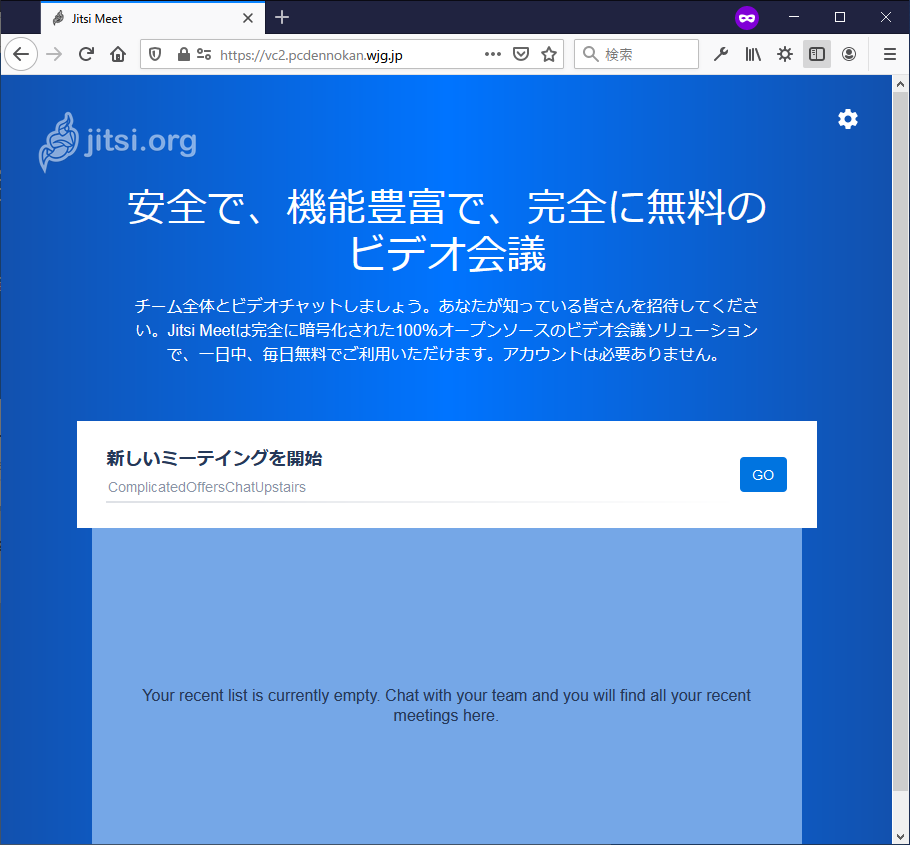
\includegraphics[keepaspectratio,width=0.6\hsize]{../2020/image202004/jitsi_web_top.png}
\end{center}
\caption{Jitsiサーバのwebのトップ画面}
\label{fig:jitsi-web-top}
\end{figure}


\subsubsubsection{(オプション設定)NAT 環境の後ろで Jitsi サーバを動かす設定}

Jitsi サーバを置くネットワーク構成によっては、サーバがグローバル IP アドレスを直接持たず NAT してインターネットに接続する構成の場合があります(GCE や Docker を利用する場合は NAT 構成になります)。その場合は jitsi-videobridge2 デーモンに設定を加える必要があります\footnote{イントラネット環境やグローバルIPを直接サーバに割り当てるネットワーク構成の場合はこの設定変更は不要です。}。

\begin{commandline}
$ sudo vi /etc/jitsi/videobridge/sip-communicator.properties
    (snip)
org.ice4j.ice.harvest.NAT_HARVESTER_LOCAL_ADDRESS=10.146.0.6
org.ice4j.ice.harvest.NAT_HARVESTER_PUBLIC_ADDRESS=34.84.236.29
    (snip)
\end{commandline}

jitsi-videobridge2 デーモンを再起動して設定を反映します。

\begin{commandline}
$ sudo systemctl restart jitsi-videobridge2
\end{commandline}

NAT設定の説明は以下 URL に情報があります。

\url{https://github.com/jitsi/jitsi-meet/blob/master/doc/quick-install.md#advanced-configuration}


\subsubsection{ビデオ会議を行う}

ここまで設定してようやく Jitsi を使ってビデオ会議ができるようになりました。

以下のURLへアクセスし、画面中央の「新しいミーティングを開始」に会議室名を入力するとビデオ会議のURLへジャンプして会議室ができます。会議に参加する方にはそのURLを連絡し、WebブラウザまたはモバイルアプリでURLを開くことで会議に参加することができます。

\begin{itemize}
\item https://vc2.pcdennokan.wjg.jp/
\end{itemize}


\subsection{Jitsiのカスタマイズについて}

\subsubsection{設定ファイルの場所}

Jitsi の設定ファイルは "/etc/jitsi" 配下及び "/usr/share/jitsi-*" 配下のディレクトリにあります。主な設定ファイルを以下に示します。

\begin{itemize}
\item /etc/jitsi/meet/vc2.pcdennokan.wjg.jp-config.js \\(インストール時に入力したDNS名を含むファイル名が生成されます)
\item /usr/share/jitsi-meet/interface\_config.js
\item /usr/share/jitsi-meet/libs/external\_api.min.js
\end{itemize}


\subsubsection{最近の会議室一覧の非表示}

Jitsi のトップ画面を開くと最近作成された会議室の一覧が表示されます。ただ、会議室の存在を知る人を制限するには誰でも会議室の URL がわかる状態になっているのは好ましくありません。

/usr/share/jitsi-meet/interface\_config.js の "RECENT\_LIST\_ENABLED" パラメータを変更すると Jitsi の最近の会議室一覧の表示をしないようにできます。

\begin{commandline}
# vi /usr/share/jitsi-meet/interface_config.js
  (snip)
  
  RECENT_LIST_ENABLED: false,

  (snip)
\end{commandline}


\subsubsection{ストリーミングのビデオの画質調整}

Jitsi のビデオ会議の画質はサーバ側で HD(720p、1280x720px)がデフォルトに設定されています\footnote{ノートPCに搭載しているWebカメラのほとんどはHD(720p、1280x720px)の品質のものが多いです。}。大変きれいなのですが、パケットの転送量が多くなるため通信帯域が細い場合に遅延が起こる、クライアントPCとJitsiサーバの負荷が高くなる、Jitsi サーバのトラフィックにかかる料金が気になる、などストリーミングならではの悩みが出てきます。

config.js の設定変更を行うとビデオ会議の画質を変更することができます。"resolution" 値はクライアント PC の Web カメラの解像度の設定値であり、"constraints" のオブジェクトの値はクライアント PC が視聴する他の参加者のビデオの画質の設定値です。

以下の config.js はクライアント PC の Web カメラの解像度の画質を「480p」とし、クライアント PC が視聴する他の参加者のビデオの画質を「480p〜240p」とする設定例です。

\begin{commandline}
# vi /etc/jitsi/meet/vc2.pcdennokan.wjg.jp-config.js
    (snip)
  
   // Sets the preferred resolution (height) for local video. Defaults to 720.
    resolution: 480,

    // w3c spec-compliant video constraints to use for video capture. Currently
    // used by browsers that return true from lib-jitsi-meet's
    // util#browser#usesNewGumFlow. The constraints are independent from
    // this config's resolution value. Defaults to requesting an ideal
    // resolution of 720p.
    constraints: {
        video: {
            height: {
                ideal: 480,
                max: 480,
                min: 240
            }
        }
    },

    (snip)
\end{commandline}

なお config.js は https://vc2.pcdennokan.wjg.jp/config.js のURLでクライアント PC へ配信されます。


\subsection{2020年3月Debian勉強会のJitsiサーバのリソース使用量}

\subsubsection{サーバ環境}

2020 年 3 月に開催したDebian 勉強会の後半は Jitsi サーバを試験的に利用して 15 名で BoF を 1 時間程度行いました。その時のサーバ環境、サーバリソースの使用量を公開します。

Jitsi サーバは以下の環境で用意していました。

\begin{itemize}
\item クラウドサービス
  \begin{itemize}
  \item Google Compute Engine (GCE)
  \end{itemize}
\item サーバのスペック
  \begin{itemize}
  \item マシンタイプ: N1 標準マシンタイプ n1-standard-1
  \item vCPU: 1 コア
  \item RAM: 3.75 GB
  \item ネットワーク下り帯域幅: 2 Gbps
  \item Disk: 10 GB
  \item OS: Debian 9 Stretch\footnote{Webの情報ではDebian 9のインストール情報が多く見つかり、時間的制約からDebian 9を選んだ経緯があります。}
  \end{itemize}
\end{itemize}

Jitsiアプリケーションのバージョンは以下でした(2020 年 4 月 18 日現在の最新版より少し古いバージョンです)。

\begin{commandline}
$ dpkg -l | grep jitsi
ii  jitsi-meet             1.0.4101-1  all    WebRTC JavaScript video conferences
ii  jitsi-meet-prosody     1.0.3729-1  all    Prosody configuration for Jitsi Meet
ii  jitsi-meet-web         1.0.3729-1  all    WebRTC JavaScript video conferences
ii  jitsi-meet-web-config  1.0.3729-1  all    Configuration for web serving of Jitsi Meet
ii  jitsi-videobridge      1126-1      amd64  WebRTC compatible Selective Forwarding Unit (SFU)
\end{commandline}


\subsubsection{CPU利用率}

サーバの CPU 利用率のグラフを 図 \ref{fig:graph_jitsi-cpu-usage} に示します。ピーク時で 86\%の使用率でした。CPU コア数は 1 コアの割り当てのため、意外と処理できていた感じがあります。

なお、当日サーバ上で top コマンドの表示を確認していたときはのロードアベレージが 6 程度だった記憶があります。

\begin{figure}[h]
\begin{center}
  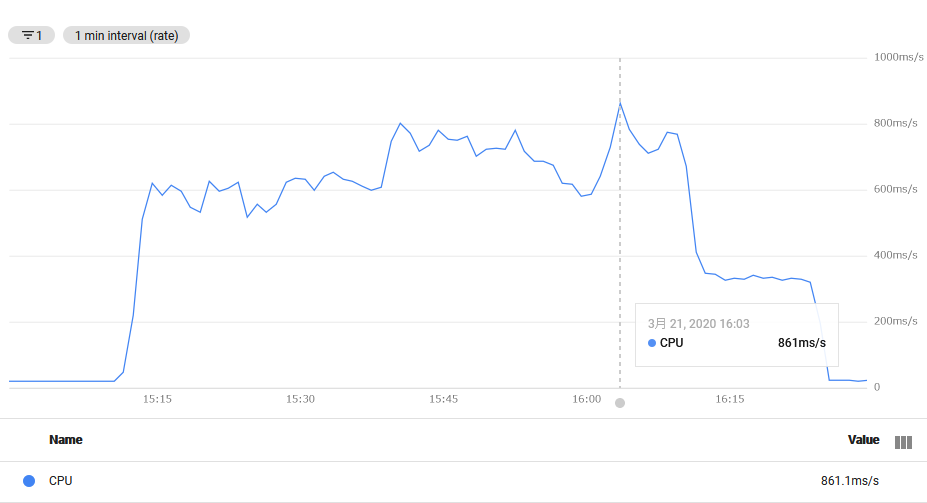
\includegraphics[keepaspectratio,width=0.75\hsize]{../2020/image202004/jitsi_perf_cpu_usage.png}
\end{center}
\caption{JitsiサーバのCPU利用率のグラフ(vCPU割り当て数:1)}
\label{fig:graph_jitsi-cpu-usage}
\end{figure}


\subsubsection{受信トラフィック}

サーバの受信(上り)トラフィックのグラフを 図 \ref{fig:graph_jitsi-traffic-recv} に示します。ピーク時で 1.653 MiB/s(= 13.22 Mbps) の受信トラフィックがあり、15 台のクライアントPCから受信したストリーミングデータの合計値となります。ただ、参加者は利用するクライアント PC の Web カメラを無効にしていた方が多く音声データのみを送信している人が多かったと推測しています。

\begin{figure}[h]
\begin{center}
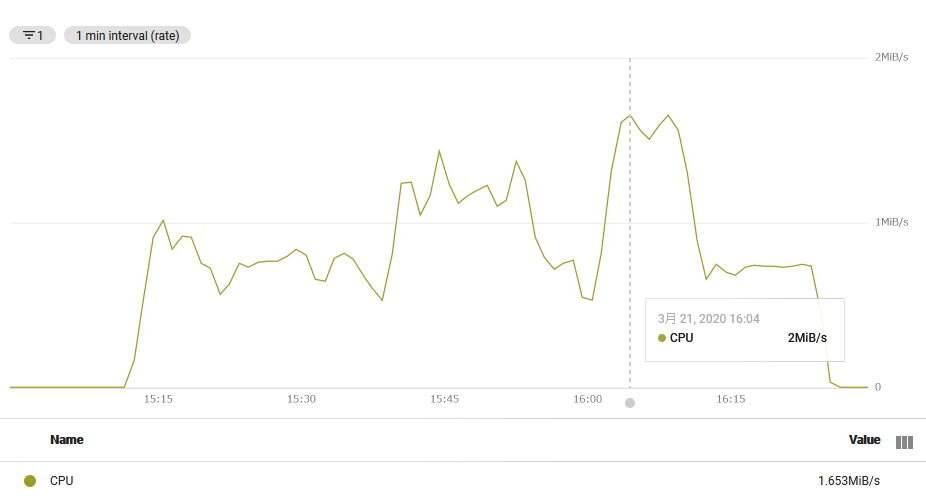
\includegraphics[keepaspectratio,width=0.75\hsize]{../2020/image202004/jitsi_perf_nw_recv-byte.png}
\end{center}
\caption{Jitsiサーバの受信トラフィックのグラフ}
\label{fig:graph_jitsi-traffic-recv}
\end{figure}


\subsubsection{送信トラフィック}

サーバの送信(下り)トラフィックのグラフを 図 \ref{fig:graph_jitsi-traffic-send} 示します。ピーク時で 6.828 MiB/s(= 54.62 Mbps) の送信トラフィックがあり、15 台のクライアント PC へ送信したストリーミングデータの合計値となります。会議の参加者の目線で見ると、参加者が利用するクライアント PC の Web カメラを無効にしていた方が多かった状態でピーク時に一人あたり 3.66 Mbps の受信トラフィックが出ていた計算となります。

仮に会議中に 55 Mbps の送信トラフィックが常に出ていると仮定した場合、1 GB の送信トラフィックを 2 分 30 秒で消費します。120 分の勉強会で利用した場合は約 48 GB の送信トラフィックが発生する計算になります。

\begin{figure}[h]
\begin{center}
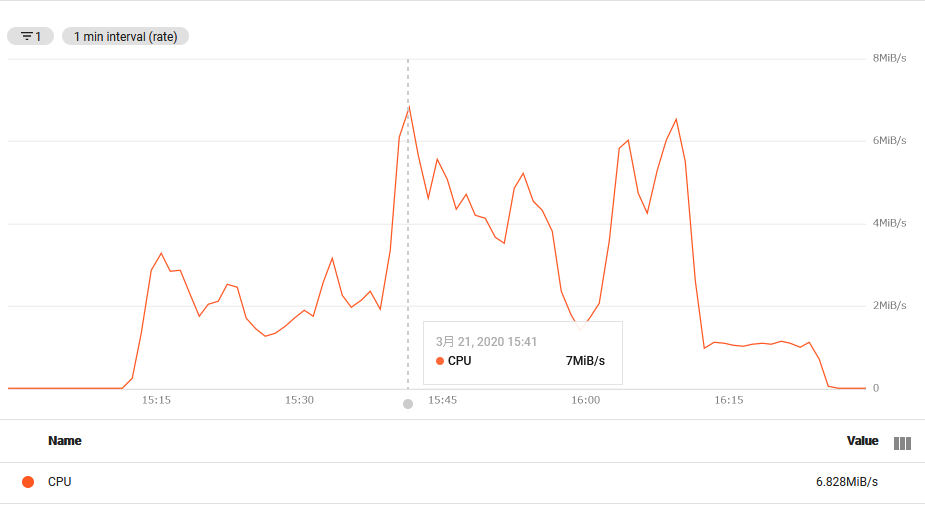
\includegraphics[keepaspectratio,width=0.75\hsize]{../2020/image202004/jitsi_perf_nw_send-byte.png}
\end{center}
\caption{Jitsiサーバの送信トラフィックのグラフ}
\label{fig:graph_jitsi-traffic-send}
\end{figure}


\subsubsection{おわりに}

Jitsi サーバを実際に構築してオンラインのビデオ会議で使ってみました。Jitsi サーバの快適な動作に必要なサーバ性能やネットワーク帯域はクライアントPCのカメラの解像度やフレームレートによっても変わってきます。自分好みの設定に調整できること、イントラネットに自分でビデオ会議サーバを作れること、そしてソースコードの書き換えもできること、これがオープンソースの醍醐味ですのでぜひとも Jitsi を利用してみてください。



%201912
%-------------------------------------------------------------------------------
\dancersection{Debian 10 busterでnftablesを使ってみる}{杉本典充}
%-------------------------------------------------------------------------------

\subsection{はじめに}

2019年7月6日にリリースした安定版Debian 10 busterではネットワークフィルタリング機能にnftablesがデフォルトで使われるように変わりました。

Debian 10 busterを使ってサーバを公開する場合にはnftablesを使うことがあると思いますので、調べてみました。


\subsection{nftableとは}

\subsubsection{nftableの歴史}

nftables\footnote{\url{https://wiki.nftables.org/wiki-nftables/index.php/Main_Page}}とは、linux-3.13 (2014/1/19リリース)から追加されたネットワークフィルタリング機能で iptables を置き換えることを目的として開発を進めている機能です。

iptables は linux-2.4 で新たに実装されたnetfilter\footnote{\url{https://www.netfilter.org/}}という機能を使ってネットワークフィルタリング処理を行う仕組みで、歴史が長いです\footnote{iptables-1.0.0.tar.bz2に含まれるmanファイル"iptables.8"には2000年3月20日という日付が入っています。}。

iptables は非常に長く多くの人たちに使われており、以下の課題があることがわかってきました\footnote{\url{https://wiki.nftables.org/wiki-nftables/index.php/Why_nftables\%3F}}。

\begin{itemize}
\item ソースコードに重複したコードが存在している
\item 性能の頭打ち
\item IPv4とIPv6のデュアルスタック時の管理の煩雑さ(nftablesのinetファミリーの追加につながる)
\item ルールセットの更新処理がアトミックでない
\item サードパーティアプリケーションが使えるAPIがない(nftablesではNetlink APIがある)
\item 構文の改善
\end{itemize}

上記を改善するため nftables の開発とlinux kernel の netfilter 機能の改善が行われ、2014年1月20日に nftables-0.099 がリリースされました\footnote{\url{https://www.netfilter.org/projects/nftables/downloads.html}}。現在の最新版は2019年12月2日にリリースした nftables-0.9.3 が最新版です。


\subsubsection{debianとnftables}

Debian においては、Debian wiki に nftables の情報があります\footnote{\url{https://wiki.debian.org/nftables}}。

Debian 9 stretch から nftables パッケージを提供しており、従来通り iptables をデフォルトとしつつ nftables も利用できる状況になっていました。このとき iptables が使う kernel module は以下になっています。

\begin{commandline}
$ cat /etc/debian_version
9.11  
$ lsmod | grep table
  ebtable_filter         16384  0
  ebtables               36864  1 ebtable_filter
  ip6table_filter        16384  0
  ip6_tables             28672  1 ip6table_filter
  iptable_filter         16384  1
  iptable_nat            16384  1
  nf_nat_ipv4            16384  1 iptable_nat
  iptable_mangle         16384  1
  ip_tables              24576  3 iptable_mangle,iptable_filter,iptable_nat
  x_tables               36864  12 ipt_REJECT,iptable_mangle,ip_tables,ebtables,iptable_filter,xt_tcpudp,
ipt_MASQUERADE,xt_CHECKSUM,ip6table_filter,xt_policy,xt_conntrack,ip6_tables
\end{commandline}

Debian 10 buster では iptables から nftables へデフォルトを切り替えており\footnote{\url{https://www.debian.org/releases/stable/amd64/release-notes/ch-whats-new.ja.html}}、nftables-0.9.0 を提供しています。nftables が使う kernel module は以下になっています。

\begin{commandline}
$ cat /etc/debian_version
10.2
$ lsmod | grep table
nf_tables_set          32768  6
nf_tables             143360  60 nft_ct,nf_tables_set
nfnetlink              16384  1 nf_tables
\end{commandline}

また、iptables パッケージの提供もしており昔ながらの使い方もできるようになっています。iptables パッケージの中には "/usr/sbin/iptables-nft" と "/usr/sbin/iptables-legacy" の二種類を提供しており、*-nft の方は nf\_tables の kernel module を使い、*-legacy の方は従来通り x\_tables の kernel module を使っています。そのため、Debian 10 busterでは、1. nf\_tables の nft インタフェース、2. nf\_tables の iptables 互換インタフェース、3. x\_tables の旧来の iptables インタフェース の3つが動作するようになっています。

Debian 11 bullseye で nftables と iptables をどうしていくかの意見がメーリングリストやブログに投稿されています。意見としては iptables パッケージを optional 扱いにして nftables パッケージのみインストールされるようにする案に賛同する人が見られます(他の意見は firewalld をデフォルトにしてはどうかという案)。

\begin{itemize}
\item default firewall utility changes for Debian 11 bullseye\footnote{\url{https://lists.debian.org/debian-devel/2019/07/msg00332.html}}
\item What to expect in Debian 11 Bullseye for nftables/iptables\footnote{\url{https://ral-arturo.org/2019/10/14/debian-netfilter.html}}
\end{itemize}


\subsection{Debian 10 busterでnftablesを使ってみる}

\subsubsection{インストール方法}

Debian 10 busterにおいて提供している nftables パッケージをインストールすると nft コマンドを利用できるようになり、nftables が systemd に登録されます。

\begin{commandline}
# apt-get install nftables
  
# which nft
/usr/sbin/nft
  
# systemctl status nftables
nftables.service - nftables
  Loaded: loaded (/lib/systemd/system/nftables.service; disabled; vendor preset: enabled)
  Active: inactive (dead)
  Docs: man:nft(8)
  http://wiki.nftables.org
\end{commandline}

nftables のパケットフィルタリングルールの設定ファイルは、/etc/nftables.conf に配置されます。初期状態では以下の設定が入っています。

\begin{commandline}
$ cat /etc/nftables.conf
#!/usr/sbin/nft -f

flush ruleset

table inet filter {
  chain input {
    type filter hook input priority 0;
  }
  chain forward {
    type filter hook forward priority 0;
  }
  chain output {
    type filter hook output priority 0;
  }
} 
\end{commandline}


\subsubsection{nftコマンドの使い方}

nftables によるネットワークフィルタリングの機能は nft コマンドで制御します。

"nft list ruleset" コマンドを実行すると現在のルールを表示します。

\begin{commandline}
# nft list ruleset
table inet filter {
    chain input {
        type filter hook input priority 0; policy accept;
    }

    chain forward {
        type filter hook forward priority 0; policy accept;
    }

    chain output {
        type filter hook output priority 0; policy accept;
    }
}
\end{commandline}

nftables へのルール定義の追加、変更、削除は以下の流れで行います。

\begin{itemize}
\item table の作成
\item chain の作成
\item rule の作成
\end{itemize}


\subsubsubsection{table の作成}

まずは最初に table を作成します。table を作成するときの引数にはアドレスファミリーを指定します。アドレスファミリーは以下表を値を指定できます\footnote{man nftより抜粋}。

\begin{table}[htb]
  \begin{center}
  \caption{nft で利用できるアドレスファミリー} 
  \begin{tabular}{|c|c|}
    \hline
    アドレスファミリー & 説明 \\ \hline
    ip & IPv4 address family. \\ \hline
    ip6 & IPv6 address family. \\ \hline
    inet & Internet (IPv4/IPv6) address family. \\ \hline
    arp & ARP address family, handling IPv4 ARP packets. \\ \hline
    bridge & Bridge address family, handling packets which traverse a bridge device. \\ \hline
    netdev & Netdev address family, handling packets from ingress. \\ \hline
  \end{tabular}
  \end{center}
\end{table}


コマンドの例です。

\begin{commandline}
# nft add table ip mytable
\end{commandline}


\subsubsubsection{chain の作成}

次に chain を作成します。chain を作成するときの引数には フックタイプ を指定します\footnote{linux kernelのNetfilter機構ではネットワークの入出力するパケットに対して任意な処理をひっかける機能がありこれを「フック」と呼んでいます。nftables や iptables は、このフック処理を設定するフロントエンドツールと言えると思います。}。前述ではip (=IPv4)を指定していますので、以下表のIPv4/IPv6/Inetのフックタイプを指定できます\footnote{man nftより抜粋。}。

\begin{table}[htb]
  \begin{center}
  \caption{nft の IPv4/IPv6/Inet で利用できるフックタイプ} 
  \begin{tabular}{|c|c|}
    \hline
    フックタイプ & 説明 \\ \hline
    prerouting & ルーティング処理の前に実行するフック \\ \hline
    input & パケットの入力時に実行するフック \\ \hline
    forward & パケットの転送時に実行するフック \\ \hline
    output & パケットの出力時に実行するフック \\ \hline
    postrouting & ルーティング処理の後に呼び出されるフック \\ \hline
  \end{tabular}
  \end{center}
\end{table}

コマンドの例です。

\begin{commandline}
# nft add chain ip mytable mychain_in { type filter hook input priority 0 \; }
\end{commandline}


\subsubsubsection{rule の作成}

次に rule を作成をします。前述の例では IPv4 の入力パケットをフィルターするchainを作成しましたのでこれに準ずるruleを作成します。以下は、外部から入力パケット はssh のみを許可し、他は拒否する設定にしてみた例です。

\begin{commandline}
# nft add rule ip mytable mychain_in tcp dport ssh accept
# nft chain ip mytable mychain_in { policy drop \; }
\end{commandline}

上述の実行する nft コマンドを見ると「tcp」「dport」「ssh」「accept」と記述しています。「tcp」の部分は udp とも書け、「dport」の部分は sport とも書け、「ssh」の部分は プロトコル名またはポート番号でもよく、「accept」の部分は drop とも書けます。これらを記述を組み合わせて自分の実現したいルールを作ってください。

細かいruleを設定するコマンドの構文は「man nft」を参照してください。


\subsubsubsection{設定の保存}

ここまで設定すると以下のようなルールで動作しています\footnote{例示のためこのようなルールになっていますが、IPv6のssh通信が外からくると通信できてしまうため本番運用するにはおそらく設定として不完全ですので注意してください。}。

\begin{commandline}
# nft list ruleset
table inet filter {
    chain input {
        type filter hook input priority 0; policy accept;
    }

    chain forward {
        type filter hook forward priority 0; policy accept;
    }

    chain output {
        type filter hook output priority 0; policy accept;
    }
}
table ip mytable {
    chain mychain_in {
        type filter hook input priority 0; policy drop;
        tcp dport ssh accept
    }
}
\end{commandline}

nftables が参照する設定ファイルは /etc/nftables.conf であり、"nft list ruleset" コマンドの出力をそのまま保存すればよいようになっています。

\begin{commandline}
# cp -p /etc/nftables.conf /etc/nftables.conf.backup1
# nft list ruleset > /etc/nftables.conf  
\end{commandline}

nftables を再起動して同じ設定が読み込まれるか確認します。

\begin{commandline}
# systemctl restart nftables
# nft list ruleset
\end{commandline}

設定に問題がなければサーバの起動時にルールを自動反映するように設定します。

\begin{commandline}
# systemctl enable nftables
\end{commandline}


\subsection{利用シーンにおける設定例}

\subsubsection{インターネットに公開するwebサーバ向け}

インターネットに公開するwebサーバでは、基本的にhttp、https、sshのポートを公開すればよいと思います。設定は以下の条件で設定してみました。

\begin{itemize}
\item 入力パケットのデフォルト処理は破棄とし、許可したルールの入力パケットのみを受信
\item ループバックインタフェースの通信はすべて許可
\item 自分のホストから通信を開始した場合の相手のサーバからの戻りパケットは受信許可
\item TCPのコネクションの状態としておかしいパケットは破棄
\item pingのエコー要求を許可
\item sshをLAN内から通信を許可
\item sshをインターネットからポート番号をtcpの10022ポートに変更した状態で通信を許可
\item http/httpsはインターネットからもLAN内からも通信を許可
\item IPv6ではssh、http/httpsのサービスはせず、ping6の応答もしない
\end{itemize}

nftables の設定は以下になります。

\begin{commandline}
# nft list ruleset
table ip filter {
    chain input {
        type filter hook input priority 0; policy drop;
        ct state { established, related } accept
        ct state { invalid } drop
        iifname "lo" accept
        icmp type { echo-reply, echo-request } accept
        tcp dport ssh ip saddr { 10.0.0.0/8, 172.16.0.0/12, 192.168.0.0/16 } accept
        tcp dport 10022 ip saddr { 0.0.0.0-255.255.255.255 } accept
        tcp dport { http, https } ip saddr { 0.0.0.0-255.255.255.255 } accept
    }

    chain forward {
        type filter hook forward priority 0; policy accept;
    }

    chain output {
        type filter hook output priority 0; policy accept;
    }
}
table ip6 filter {
    chain input {
        type filter hook input priority 0; policy drop;
        iifname "lo" accept
    }

    chain forward {
        type filter hook forward priority 0; policy accept;
    }

    chain output {
        type filter hook output priority 0; policy accept;
    }
}
\end{commandline}


\subsubsection{インターネットに公開するopenvpnサーバ向け}

openvpn\footnote{\url{https://openvpn.net/community/}} とは SSL-VPN の機能をもった VPN サーバ及び VPN クライアントアプリケーションです。openvpn を使って VPN 接続したクライアントは openvpn サーバを中継して別のネットワークのサーバと通信することができます。

ここでは openvpn に接続したサーバ及びクライアントに割り当てられるネットワークアドレス帯"192.168.200.0/24"からパケットが入力された場合に、他のネットワークへパケットをルーティングする設定を行います。

\begin{commandline}
# nft add table ip nat
# nft add chain ip nat postrouting { type nat hook postrouting priority 100 \; }
# nft add rule ip nat postrouting oifname "eth0" ip saddr 192.168.200.0/24 masquerade 
\end{commandline}

openvpnを起動すると追加される"tun"インタフェースについても受信許可し、openvpnが利用するUDPとTCPの 1194 番ポートの通信を受信許可に設定します。

nftables の設定は以下になります。

\begin{commandline}
# nft list ruleset
table ip filter {
    chain input {
        type filter hook input priority 0; policy drop;
        ct state { established, related } accept
        ct state { invalid } drop
        iifname "lo" accept
        iifname "tun*" accept
        icmp type { echo-reply, echo-request } accept
        tcp dport ssh ip saddr { 10.0.0.0/8, 172.16.0.0/12, 192.168.0.0/16 } accept
        tcp dport 10022 ip saddr { 0.0.0.0-255.255.255.255 } accept
        udp dport openvpn ip saddr { 0.0.0.0-255.255.255.255 } accept
        tcp dport openvpn ip saddr { 0.0.0.0-255.255.255.255 } accept
    }

    chain forward {
        type filter hook forward priority 0; policy accept;
    }

    chain output {
        type filter hook output priority 0; policy accept;
    }
}
table ip6 filter {
    chain input {
        type filter hook input priority 0; policy drop;
        iifname "lo" accept
    }

    chain forward {
        type filter hook forward priority 0; policy accept;
    }

    chain output {
        type filter hook output priority 0; policy accept;
    }
}  
table ip nat {
    chain postrouting {
        type nat hook postrouting priority 100; policy accept;
        oifname "eth0" ip saddr 192.168.200.0/24 masquerade
    }
}
\end{commandline}


\subsection{おわりに}

Debian 10 でデフォルトになった nftables を調べてみました。

今後 nftables が主流になっていくと思われるため Debian 10 buster を使い始める方は nftables も合わせて使い始めてみてはいかがでしょうか。 


\subsection{参考文献}

\begin{itemize}
\item 「nftables - Debian Wiki」 \url{https://wiki.debian.org/nftables}
\item 「netfilte.org」 \url{https://www.netfilter.org/}
\item 「netfilter wiki」 \url{https://wiki.nftables.org/wiki-nftables/index.php/Main_Page}
\item 「Linuxにおける新たなパケットフィルタリングツール「nftables」入門 - さくらのナレッジ」 \url{https://knowledge.sakura.ad.jp/22636/}
\item 「nftables で基本的なフィルタリングを設定してみた - SIOS TECH.LAB」 \url{https://tech-lab.sios.jp/archives/16930}
\end{itemize}

%202005
\dancersection{Debian パッケージリポジトリの作成・管理ツール aptly}{岩松 信洋}
%-------------------------------------------------------------------------------

Debian パッケージリポジトリのミラー作成、独自のパッケージリポジトリ作成などを
サポートするツール、aptlyについて説明します。

\subsection{aptly とは}

aptly (\url{https://www.aptly.info/}) は Debian パッケージリポジトリの作成・管理するツールの一つです。
パッケージリポジトリの作成やミラーリングを行うツールとして、dpkg-dev、apt-ftparchive、reprepro、archvsync などがありますが、
これらは機能が限定的であり、いくつかのツールを組み合わせて使うことがほとんどです。aptly はこれらをまとめた
機能を提供しています。

\begin{itemize}
\item パッケージリポジトリのフルミラーリングおよびフィルターミラーリング(アーキテクチャー、コンポーネント、パッケージ)
\item パッケージリポジトリのスナップショット作成
\item  パッケージリポジトリの更新、マージ、リリース
\item パッケージリポジトリサーバー機能
\item ローカルパッケージリポジトリの作成
\item パッケージリポジトリ操作用 REST APIの提供
\item Amazon S3 などのクラウドストレージへのアップロード機能
\end{itemize}

コマンドが統一されており、REST API も提供されていることから、CIやCDと親和性が高く、パッケージやパッケージを使った
製品のテスト等に役立ちます。
またスナップショット機能があり、スナップショットをベースにパッケージリポジトリを構築するため、構成管理や組込み機器
のルートファイルシステムの管理などにも利用できます。

\subsubsection{aptly の構成要素}

aptly の構成要素としてはミラーリポジトリ、ローカルパッケージリポジトリ、スナップショットリポジトリ、パッケージ
リポジトリの4つに分類され、前の3つで提供されるパッケージ情報を使って、公開するパッケージリポジトリ
を作成することになります。

\begin{itemize}
\item ミラーリポジトリ

ミラーリポジトリはDebianパッケージを提供しているパッケージリポジトリをミラーしたものを指します。
Debian パッケージなので、Debian の公式・非公式関係なくミラーできます。またUbuntu のリポジトリや PPA からも
ミラーを構築できます。

\item ローカルパッケージリポジトリ

ローカルパッケージリポジトリは、独自に作成したDebian パッケージ用リポジトリを管理する場合に使用します。

\item スナップショット

ローカルパッケージリポジトリとミラーリポジトリのスナップショットを作成します。
Debianの公式リポジトリを直接参照している場合、対処のパッケージが更新されると、古いバージョンのパッケージが
対象リポジトリ参照できなくなり、同じパッケージ構成を持つマシンなどを構成することが難しくなります。
このような場合、ある時点のパッケージ情報をスナップショットとして
保存するなどの対策する必要があるのですが、aptly のリポジトリスナップショット機能を使うと、容易に実現できます。

\item パッケージリポジトリ

ミラーリポジトリ、ローカルパッケージリポジトリ、スナップショットは aptly で管理されるデータベース上で
管理されます。これらを組みわせて作成したリポジトリデータを元にパブリッシュ(公開)することで初めてパッケージリポジトリ
として利用できるようになります。

\end{itemize}


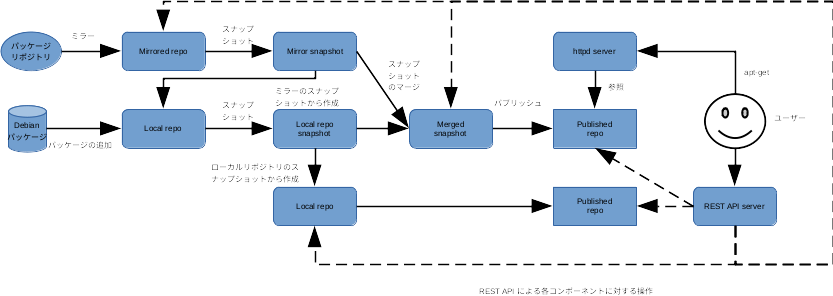
\includegraphics[width=1.0\hsize]{../2020/image202005/aptly-image00.png}

\begin{itemize}
\item ミラーリポジトリは他のパッケージリポジトリから作成します。
\item  ローカルパッケージはパッケージを追加するか、ローカルミラーから作成できます。
\item  作成したローカルミラーやローカルリポジトリはそのままではパッケージリポジトリとしては利用できず、パブリッシュ(公開)する必要があります。
\item  ローカルミラーやローカルリポジトリはスナップショットを作成できます。
\item  スナップショットからスナップショットも作成でき、スナップショット同士の依存関係もメタデータとして管理されます。
\item  スナップショット同士でマージできます。
\item  パプリッシュしたパッケージリポジトリは aptly で提供される httpサーバー、またはその他httpサーバーを使って公開できます。
\end{itemize}

\subsubsection{aptly を使用する際に注意すること}

aptly ではパッケージリポジトリを公開する場合に、GnuPGによる署名が必要となります(必須ではなく、オプションで署名および
確認を無視できます)。aptly は一度ローカルにパッケージとメタ情報を保存し、
それらを組み合わせて、パッケージリポジトリに必要なReleaseファイルなどのメタデータを再構築
します。再構築したメタデータはフルミラーであっても内容が異なるため、正しくパッケージリポジトリ
を運用するにはこれらに GnuPG による署名が必要になります。
メタデータを含めたフルミラーを構築したい場合は archvsync (\url{https://salsa.debian.org/mirror-team/archvsync}) 
や apt-mirror パッケージを使うと良いでしょう。

またパッケージリポジトリの構築にはハードリンクを使います。よってハードリンクの制限が適用されることに注意
が必要です。Amazon S3 などのクラウドストレージにパッケージリポジトリをパブリッシュする際にはこの制限はありません。

以下からは、aptly に使い方について説明します。

\subsection{aptly のインストール}

aptlyは公式Debianパッケージとして提供されています。執筆時のDebianパッケージバージョンは 1.3.0+ds1-4 となっています。
以下のコマンドでインストールできます。

\begin{commandline}
$ sudo apt update
$ sudo apt install aptly
\end{commandline}

また Upstream のバージョンは 1.4.0 となっており、GnuPG 2.x へのサポート強化などが行われています。
最新バージョンを使いたい場合には、以下のようにアップストリーム が提供するリポジトリで提供されている
パッケージが利用できます。 ディストリビューション部が squeeze となっていますが、一つのディストリビューション
のみで提供されているので、気にしなくても良いです。

\begin{commandline}
$ wget -qO - https://www.aptly.info/pubkey.txt | sudo apt-key add -
$ sudo sh -c "echo deb http://repo.aptly.info/ squeeze main > /etc/apt/sources.list.d/aptly.list"
$ sudo apt update
$ sudo apt install aptly
\end{commandline}

\subsubsection{aptly の設定}

aptly の設定は \$HOME/.aptly.confに記載されています。
内容は aptly config コマンドの show サブコマンドで確認できます。
もちろん普段お使いのエディタ等で確認してもかまいません。

\begin{commandline}
$ aptly config show
{
    "rootDir": "/home/aptly/.aptly",
    "downloadConcurrency": 4,
    "downloadSpeedLimit": 0,
    "architectures": [],
    "dependencyFollowSuggests": false,
    "dependencyFollowRecommends": false,
    "dependencyFollowAllVariants": false,
    "dependencyFollowSource": false,
    "dependencyVerboseResolve": false,
    "gpgDisableSign": false,
    "gpgDisableVerify": false,
    "gpgProvider": "gpg",
    "downloadSourcePackages": false,
    "skipLegacyPool": true,
    "ppaDistributorID": "ubuntu",
    "ppaCodename": "",
    "skipContentsPublishing": false,
    "FileSystemPublishEndpoints": {},
    "S3PublishEndpoints": {},
    "SwiftPublishEndpoints": {}
}
\end{commandline}

詳細は省きますが、重要なのは rootDir の項目で、ここで指定されるディレクトリにaptly が管理する
パッケージのメタデータやローカルパッケージリポジトリ等が格納されます。
また Amazon S3 や OpenStack Swift へのアップロードを行う際には、S3PublishEndpointsやSwiftPublishEndpointsに対して
アクセスキー等を設定します。
各項目の詳細は Configuration (\url{https://www.aptly.info/doc/configuration/}) を確認してください。

\subsection{GnuPG 鍵の作成とパッケージリポジトリの署名確認必要な公開鍵のインポート}

aptly を使う前に、GnuPG鍵の作成と、パッケージミラー元のGnuPG公開鍵をインポートする
必要があります。
前述したように、正しくパッケージリポジトリを運用するにはGnuPGによる署名が必要なため、
GnuPG鍵を作成します。既にGnuPG鍵を持っている場合も、リポジトリ管理用に別途GnuPG鍵を
作成しておくとよいでしょう。GnuPG鍵の作成には以下のように実行します。

\begin{commandline}
$ gpg --gen-key

<中略>

本名: aptly
電子メール・アドレス: aptly@example.com
次のユーザIDを選択しました:
    "aptly <aptly@example.com>"

<中略>
公開鍵と秘密鍵を作成し、署名しました。

pub   rsa3072 2020-05-01 [SC] [有効期限: 2022-05-01]
      E67BDF3221F4CDFD47F4A3639A64752708B70EFA
uid                      aptly <aptly@example.com>
sub   rsa3072 2020-05-01 [E] [有効期限: 2022-05-01]
\end{commandline}

次にパッケージミラー元の GnuPG公開鍵をインポートします。
パッケージリポジトリのミラー元の情報を取得する際にミラー元の署名を確認する必要があるためです。
Debian のオフィシャルパッケージリポジトリを使う場合には以下のように実行します。

\begin{commandline}
$ sudo apt install debian-archive-keyring
$ gpg --no-default-keyring --keyring /usr/share/keyrings/debian-archive-keyring.gpg --export | \
        gpg --no-default-keyring --keyring trustedkeys.gpg --import
\end{commandline}

次に Debian で提供されているパッケージを使っている人は、GnuPG v2 で作成した鍵を v1 に変換する必要があります。
これは Debian のパッケージが GnuPG v1 に依存しているためです。
公開鍵 E67BDF3221F4CDFD47F4A3639A64752708B70EFA をコンバートし、GnuPG v1 にインポートする方法を
以下に示します。

\begin{commandline}
$ gpg --output gpg2_export_pub.gpg --armor --export E67BDF3221F4CDFD47F4A3639A64752708B70EFA
$ gpg --output gpg2_export_sec.gpg --armor --export-secret-key E67BDF3221F4CDFD47F4A3639A64752708B70EFA
$ gpg1 --import gpg2_export_pub.gpg
gpg: 鍵08B70EFA: 公開鍵"aptly <aptly@example.com>"をインポートしました
gpg:           処理数の合計: 1
gpg:             インポート: 1  (RSA: 1)
gpg: 最小の「ある程度の信用」3、最小の「全面的信用」1、PGP信用モデル
gpg: 深さ: 0  有効性:   1  署名:   0  信用: 0-, 0q, 0n, 0m, 0f, 1u
gpg: 次回の信用データベース検査は、2022-05-01です
$ gpg1 --import --allow-secret-key-import gpg2_export_sec.gpg
gpg: 鍵08B70EFA: 秘密鍵をインポートしました
gpg: 鍵08B70EFA:"aptly <aptly@example.com>"変更なし
gpg:           処理数の合計: 1
gpg:               変更なし: 1
gpg:       秘密鍵の読み込み: 1
gpg:     秘密鍵のインポート: 1
\end{commandline}

また作成するパッケージリポジトリにアクセスするマシンにパッケージリポジトリの公開鍵を登録することを
忘れないようにしましょう。公開鍵の出力方法と出力した公開鍵を登録する方法を以下に示します。

\begin{commandline}
$ gpg --export --armor > aptly.pub
\end{commandline}

\begin{commandline}
$ sudo apt-key add aptly.pub
\end{commandline}

\subsection{パッケージミラーリポジトリの作成}

ローカルにパッケージミラーリポジトリを作成する場合、 aptly mirror コマンドの create サブコマンドを使用します。
コマンドにローカルで利用する名前(name)、リポジトリのURL、ディストリビューション、コンポーネントを指定します。
例えば、

\begin{itemize}
	\item 名前: debian-buster
	\item リポジトリURL: http://deb.debian.org/debian/
	\item ディストリビューション: buster
	\item コンポーネント: main
	\item アーキテクチャ: すべて
\end{itemize}

上記のようなパッケージミラーリポジトリを作成する場合、以下のように実行します。
実行するとリポジトリが初期化されます。

\begin{commandline}
$ aptly mirror create debian-buster http://deb.debian.org/debian/ buster main
\end{commandline}

作成したパッケージミラーリポジトリの情報は list サブコマンドで
確認できます。

\begin{commandline}
$ aptly mirror list
List of mirrors:
 * [debian-buster]: http://deb.debian.org/debian/ buster

To get more information about mirror, run `aptly mirror show <name>`.
\end{commandline}

また詳細な情報が必要な場合は show サブコマンドで確認できます。

\begin{commandline}
$ aptly mirror show debian-buster
Name: debian-buster
Archive Root URL: http://deb.debian.org/debian/
Distribution: buster
Components: main
Architectures: amd64, arm64, armel, armhf, i386, mips, mips64el, mipsel, ppc64el, s390x
Download Sources: no
Download .udebs: no
Last update: never

Information from release file:
Acquire-By-Hash: yes
Architectures: amd64 arm64 armel armhf i386 mips mips64el mipsel ppc64el s390x
Changelogs: http://metadata.ftp-master.debian.org/changelogs/@CHANGEPATH@_changelog
Codename: buster
Components: main contrib non-free
Date: Sat, 09 May 2020 09:51:02 UTC
Description:  Debian 10.4 Released 09 May 2020

Label: Debian
Origin: Debian
Suite: stable
Version: 10.4
\end{commandline}

まだこの状態ではリポジトリのメタデータやパッケージがない状態のため、ミラー元から取得する必要があります。
取得するには update サブコマンドを実行します。
実行するとメタデータを取得し、パッケージのミラーを開始します。

\begin{commandline}
$ aptly mirror update debian-buster
\end{commandline}

上記では指定したディストリビューションのコンポーネントをすべてミラーします。
特定のアーキテクチャのみや、ミラーしたいパッケージを指定したい場合には、オプションを使うことで
制御できます。よく利用されるオプションを以下に示します。

\begin{itemize}
	\item アーキテクチャを指定する: -architectures
	\item パッケージをフィルターする: -filter
	\item フィルターで指定されたパッケージに依存するパッケージもミラーする: -filter-with-deps
	\item ソースパッケージもミラーする: -with-sources
\end{itemize}

アーキテクチャをamd64 と arm64、ミラーするパッケージを busybox、依存するパッケージとソースパッケージもミラーする場合
には以下のように実行します。

\begin{commandline}
$ aptly mirror create -architectures=amd64,arm64 -filter='busybox' \
    -filter-with-deps -with-sources busybox-mirror http://deb.debian.org/debian/ buster main
\end{commandline}

実行し、取得したパッケージは \$HOME/.aptly ディレクトリ以下に保存されます。
ファイルの配置は git リポジトリの .git/objects 以下のような配置になっています。

\begin{commandline}
.aptly
├── db
│ ├── 000004.ldb
│ ├── 000007.ldb
│ ├── 000008.log
│ ├── CURRENT
│ ├── LOCK
│ ├── LOG
│ └── MANIFEST-000009
└── pool
    ├── 1b
    │ └── 00
    │     └── f7cef567645a7e695caf6c1ad395_gcc-8-base_8.3.0-6_amd64.deb
    ├── 1e
    │ └── 32
    │     └── ea742bddec4ed5a530ee2f423cdf_busybox_1.30.1-4_amd64.deb
<省略> 
\end{commandline}

作成したミラーで提供されるパッケージを確認するには aptly mirror コマンドの search サブコマンド使用します。
検索するミラー名と検索用のクエリーを指定し、実行します。以下に パッケージ名が busy\* 、アーキテクチャが
arm64 であるパッケージを検索するには以下のように実行します。検索用クエリーを指定しない場合は提供されるパ
ッケージが全て出力されます。

\begin{commandline}
$ aptly mirror search busybox-mirror 'Name (% busy*), $Architecture (arm64)'
busybox_1:1.30.1-4_arm64
busybox-static_1:1.30.1-4_arm64
\end{commandline}

\subsection{ローカルパッケージリポジトリの作成}

ローカルパッケージリポジトリは、独自で作成したパッケージをリポジトリで管理したい場合などに使用します。
まず管理するためのリポジトリを作成する必要があります。
リポジトリを作成するには、aptly repo コマンド のcreate サブコマンドに作成するリポジトリ名を指定して実行します。
このリポジトリ名は Debian パッケージで利用される ディストリビューション名 (unstable, buster など)
と紐付けられています。

\begin{commandline}
$ aptly repo create my-repo
\end{commandline}

またローカルリポジトリを作成する場合、スナップショットからも作成できます。

\begin{commandline}
$ aptly repo create my-repo from snapshot snapshot-name
\end{commandline}

\subsubsection{ローカルパッケージリポジトリへのパッケージの追加}

create サブコマンドで作成した段階では、ローカルパッケージリポジトリにまだパッケージが登録されていない状態なので、
パッケージを追加します。追加する方法は以下の方法があります。

\subsubsubsection{add サブコマンドを使ったパッケージの追加}

add サブコマンドは 特定のdebian バイナリパッケージ、またはdsc (Debian source control file)を元にソースパッケージを追加
したい場合に利用します。
パッケージを指定してローカルパッケージリポトリに追加したい場合は、add サブコマンドにパッケージファイルのパスを指定して実行します。

\begin{commandline}
$ aptly repo add my-repo pool/liblz4-1_1.9.2-2_amd64.deb
Loading packages...
[+] liblz4-1_1.9.2-2_amd64 added
\end{commandline}

またソースパッケージを追加したい場合には dsc ファイルを指定して実行します。

\begin{commandline}
$ aptly repo add my-repo pool/lz4_1.9.2-2.dsc
Loading packages...
[+] lz4_1.9.2-2_source added
\end{commandline}

特定のディレクトリにあるパッケージすべて追加したい場合には対象のディレクトリを指定すればよいです。
以下の例ではpool ディレクトリを対象ディレクトリとして指定しています。

\begin{commandline}
$ aptly repo add my-repo pool
Loading packages...
[+] liblz4-1-dbgsym_1.9.2-2_amd64 added
[+] liblz4-1_1.9.2-2_amd64 added
[+] liblz4-dev_1.9.2-2_amd64 added
[+] liblz4-tool_1.9.2-2_all added
[+] lz4-dbgsym_1.9.2-2_amd64 added
[+] lz4_1.9.2-2_source added
[+] lz4_1.9.2-2_amd6 added
\end{commandline}

add コマンドを使った場合、ファイルのサイズやファイルハッシュ値の確認は行われないため注意が必要です。
より安全にパッケージをリポジトリに追加したい場合、次で説明する include サブコマンドを使います。

\subsubsubsection{include サブコマンドを使ったパッケージの追加}

ローカルパッケージリポジトリへのパッケージの追加には add サブコマンドの他にinclude サブコマンドも利用可能です。
add サブコマンドとの違いは処理の対象が .changes ファイルである事です。
.changes ファイルを指定して実行するには以下のように実行します。実行すると、.changes ファイルに記載されているパッケージ
が登録されます。特に指定しない場合、実行後にはパッケージファイル等は削除されてしまうので、削除したくない場合には
-no-remove-files オプションを指定する必要があります。
また.changes にGnuPGによる署名を行っておらず、署名の有無を無視したい場合には -accept-unsigned オプションを
指定する必要があります。

\begin{commandline}
Format: 1.8
Date: Tue, 12 Nov 2019 07:58:47 +0900
Source: lz4

<中略>

Checksums-Sha1:
 44348438b55dc32132df8039513a57c4c1cd87a5 1073 lz4_1.9.2-2.dsc
 3790bc3c9e6d4e26e5063855cf847f5af91d8420 12712 lz4_1.9.2-2.debian.tar.xz
 ce4d29ed984de507203d917e671c1894c9778e8c 323008 liblz4-1-dbgsym_1.9.2-2_amd64.deb
 aed6d84f4636d37cd94b90e9ce0320dee853eca6 57148 liblz4-1_1.9.2-2_amd64.deb
 018ef0f8bf34411b4b928072f5c1f2d1abf8103f 76752 liblz4-dev_1.9.2-2_amd64.deb
 bf32ee9eee03ef69d6b0526bed92dcc95af57883 5088 liblz4-tool_1.9.2-2_all.deb
 39f1aa1950030608ad528a4f4fe951b37e0e4956 410216 lz4-dbgsym_1.9.2-2_amd64.deb
 dec576464d1c5e4b2b69e59ab29208f4e6d741eb 6648 lz4_1.9.2-2_amd64.buildinfo
 689287ecea701b76f99c5d30040ca584bdc58fde 84076 lz4_1.9.2-2_amd64.deb

<省略>
\end{commandline}
 
\begin{commandline}
$ aptly repo include -repo my-repo pool/lz4_1.9.2-2_amd64.changes
Loading repository my-repo for changes file lz4_1.9.2-2_amd64.changes...
[+] liblz4-1-dbgsym_1.9.2-2_amd64 added
[+] liblz4-1_1.9.2-2_amd64 added
[+] liblz4-dev_1.9.2-2_amd64 added
[+] liblz4-tool_1.9.2-2_all added
[+] lz4-dbgsym_1.9.2-2_amd64 added
[+] lz4_1.9.2-2_source added
[+] lz4_1.9.2-2_amd64 added
\end{commandline}
%<!-- $ aptly repo include -repo my-repo -no-remove-files -accept-unsigned pool/lz4_1.9.2-2_amd64.changes -->

上記では実行する際に、-repo オプションでリポジトリ名を指定しています。
これは changelog で指定されているディストリビューション名(unstable など)がリポジトリ名と合致しない場合
にエラーになるためです。

またディレクトリを指定する場合には、.changes が格納されているデレクトリを指定します。

\begin{commandline}
$ aptly repo include -repo my-repo pool
Loading repository my-repo for changes file lz4_1.9.2-2_amd64.changes...
[+] liblz4-1-dbgsym_1.9.2-2_amd64 added
[+] liblz4-1_1.9.2-2_amd64 added
[+] liblz4-dev_1.9.2-2_amd64 added
[+] liblz4-tool_1.9.2-2_all added
[+] lz4-dbgsym_1.9.2-2_amd64 added
[+] lz4_1.9.2-2_source added
[+] lz4_1.9.2-2_amd64 added
\end{commandline}

指定したディレクトリに .changes ファイルがない場合や、.changes の内容が異なる場合には
処理されません。

\begin{commandline}
$ aptly repo include -repo my-repo -no-remove-files -accept-unsigned pool
[!] unable to process file lz4_1.9.2-2_amd64.changes: size mismatch: expected 12712 != obtained 12568 
[!] Some files were skipped due to errors:
  pool/lz4_1.9.2-2_amd64.changes
ERROR: some files failed to be added
\end{commandline}


% リポジトリのアップローダーを固定したい場合は**-uploaders-file=**を使う。
% uploaders のフォーマットは https://www.aptly.info/doc/aptly/repo/include/ に書いてある。

\subsubsubsection{ローカルミラーからの追加}

aptly mirror コマンドによって作成したローカルミラーで提供されているパッケージも
ローカルリポジトリに追加できます。この場合 import サブコマンドを利用します。

例えば、ローカルミラー busybox-mirror にある busybox で始まるパッケージを my-repo ローカル
リポジトリに追加する場合には以下のように実行します。

\begin{commandline}
$ aptly repo import busybox-mirror my-repo busybox
Loading packages...
[o] busybox_1:1.30.1-4_source imported
[o] busybox-static_1:1.30.1-4_amd64 imported
[o] busybox_1:1.30.1-4_arm64 imported
[o] busybox_1:1.30.1-4_amd64 imported
[o] busybox-static_1:1.30.1-4_arm64 imported
\end{commandline}

Package Queries(\url{https://www.aptly.info/doc/feature/query/})
にパッケージ名の指定方法等に関する説明があるので興味のある方は参照してください。

\subsubsection{ローカルパッケージリポジトリの削除}

ローカルパッケージリポジトリの情報を削除したい場合には、drop サブコマンドに削除したいリポジトリ名を指定します。

\begin{commandline}
$ aptly repo drop my-repo
\end{commandline}

\subsubsection{その他ローカルリポジトリに関する操作}

\begin{itemize}
\item repo list

  作成されたリポジトリのリストを出力します。

\item repo copy

  リポジトリにあるパッケージを指定したリポジトリにコピーします。
  コピー先のリポジトリは先に作成する必要があるので注意してください。

\begin{commandline}
  $ aptlu repo create my-repo-next
  $ aptly repo copy my-repo my-repo-next 'Name (%lib*)'
  Loading packages...
  [o] liblz4-tool_1.9.2-2_all copied
  [o] liblz4-1_1.9.2-2_amd64 copied
  [o] liblz4-1-dbgsym_1.9.2-2_amd64 copied
  [o] liblz4-dev_1.9.2-2_amd64 copied
\end{commandline}

\item repo move

  リポジトリにあるパッケージを指定したリポジトリに移動します。
  コピー先のリポジトリは先に作成しておく必要がある点に注意が必要です。

\item repo remove

  指定したパッケージをリポジトリから削除します。

\item repo search

  リポジトリで提供されているパッケージを検索します。

\item repo edit

  リポジトリに関する情報を修正します。

\item repo rename

  リポジトリ名を変更します。

\end{itemize}

\subsection{スナップショット}

aptly mirror update コマンドを実行した場合、ミラー元のパッケージ情報等と完全に同期するため、
ミラー元で削除されたパッケージはローカルミラーでも削除され、更新されたパッケージも古いものは
残っていない状態になります`。
またローカルパッケージリポジトリでも運用によっては上記と同じようなことが起こる可能性も
あります。このような事が起きても困らないようにするために、スナップショットを作成し、
リポジトリ内容が変化しないよう管理します。

\subsubsection{スナップショットの作成と確認}

スナップショットを作成するには、aptly snapshot コマンドの create サブコマンドを使用します。
例えば、ローカルミラー buster-mirror のスナップショットを buster-mirror-2020512 として作成するには
以下のように実行します。

\begin{commandline}
$ aptly snapshot create buster-mirror-2020512 from mirror buster-mirror
\end{commandline}

スナッショットは ローカルリポジトリからも作成できます。
ローカルリポジトリ my-repo のスナップショットを my-repo-20200512 として作成するには以下のように
実行します。

\begin{commandline}
$ aptly snapshot create imy-repo-20200510 from repo my-repo
\end{commandline}

現在作成されているスナップショットを確認するには list サブコマンド、
スナップショットの情報を確認するにはは show サブコマンドを使います。

\begin{commandline}
$ aptly snapshot list
List of snapshots:
 * [busybox-buster-mirror-20200512]: Snapshot from mirror [busybox-buster-mirror]: http://deb.debian.org/debian/ buster
 * [my-repo-20200512]: Snapshot from local repo [my-repo]

To get more information about snapshot, run `aptly snapshot show <name>`.
$ aptly snapshot show my-repo-20200512
Name: my-repo-20200512
Created At: 2020-05-15 07:06:32 UTC
Description: Snapshot from local repo [my-repo]
Number of packages: 12
Sources:
  my-repo [local]
\end{commandline}

\subsubsection{スナップショットのマージ}

作成したスナップショットをマージし、新しいスナップショットを作成するには merge サブコマンドを使います。
作成したいスナップショット名にマージするスナップショットを指定します。

\begin{commandline}
$ aptly snapshot merge my-product-release-20200512 my-repo-20200512 busybox-buster-mirror-20200512

Snapshot my-product-release-20200512 successfully created.
You can run 'aptly publish snapshot my-product-release-20200512' to publish snapshot as Debian repository.
$ aptly snapshot list
List of snapshots:
 * [busybox-buster-mirror-20200512]: Snapshot from mirror [busybox-buster-mirror]: http://deb.debian.org/debian/ buster
 * [my-product-release-20200512]: Merged from sources: 'my-repo-20200512', 'busybox-buster-mirror-20200512'
 * [my-repo-20200512]: Snapshot from local repo [my-repo]

To get more information about snapshot, run `aptly snapshot show <name>`.

$ aptly snapshot show my-product-release-20200512
Name: my-product-release-20200512
Created At: 2020-05-15 07:20:35 UTC
Description: Merged from sources: 'my-repo-20200512', 'busybox-buster-mirror-20200512'
Number of packages: 15
Sources:
  my-repo-20200512 [snapshot]
  busybox-buster-mirror-20200512 [snapshot]
\end{commandline}

\subsubsection{スナップショットの検証}

スナップショットの状態によってはパッケージの依存関係が維持できてない場合があります。
これはパッケージの追加し忘れや、ローカルミラーリポジトリを
構築した際に -filter-with-deps オプションを付けていなかったことなどが原因となります。
このような状態を確認するために、スナップショット内容を検証するサブコマンド verify が
用意されています。
以下では、-filter-with-deps を付けずに busyboxから始まるパッケージのミラーを作成し、
そのスナップショットを検証した結果です。結果(Missing dependencies (1):)からこのスナップショットでは libc6 (>= 2.28) が
不足していることがわかります。

\begin{commandline}
$ aptly mirror create -architectures=amd64 -filter='busybox' \
    busybox-buster-mirror-without-dep http://deb.debian.org/debian/ buster main
$ aptly mirror update busybox-buster-mirror-without-dep
$ aptly snapshot create busybox-buster-mirror-without-dep-v1 from mirror busybox-buster-mirror-without-dep
$ aptly snapshot verify busybox-buster-mirror-without-dep-v1
Loading packages...
Verifying...
Missing dependencies (1):
  libc6 (>= 2.28) [amd64]
\end{commandline}

このような場合、足りないパッケージを提供するリモートパッケージリポジトリを apt-line に追加するなどで対応できますが、
このリモートパッケージリポジトリの内容が変更される可能性も考えられます。根本的に問題を回避するためには、同じスナップショット
内で提供できるようにしたほうがよいでしょう。
スナップショットのベースとなったミラーを -filter-with-deps 付加した後更新し、再度スナップショットを作成するか、
他のスナップショットで必要とするパッケージが提供されているなら、次で説明する pull サブコマンドを使って、他のスナップショットから
パッケージを取り込むこともできます。

\begin{commandline}
$ aptly mirror edit -filter-with-deps busybox-buster-mirror-without-dep
$ aptly mirror show busybox-buster-mirror | grep '^Filter With Deps'
Filter With Deps: yes
$ aptly mirror update busybox-buster-mirror
\end{commandline}

\subsubsubsection{他のスナップショットからパッケージを取り込み、新しいスナップショットを作成する}

既存のスナップショットに、他のスナップショットで提供されるパッケージを取り込み、新しいスナップショット
を作成するには、pull サブコマンドを使います。
ベースとするスナップショット busybox-buster-mirror-without-dep-v1 に スナップショット libc-dev-mirror-20200512 で
提供される libc6 パッケージを取り込み、スナップショット busybox-buster-mirror-v1 を作成するには、以下のように実行
します。

\begin{commandline}
$ aptly snapshot pull busybox-buster-mirror-without-dep-v1 libc-dev-mirror-20200512 busybox-buster-mirror-v1 libc6
Dependencies would be pulled into snapshot:
    [busybox-buster-mirror-without-dep-v1]: Snapshot from mirror [busybox-buster-mirror-without-dep]: \
	http://deb.debian.org/debian/ buster
from snapshot:
    [libc-dev-mirror-20200512]: Snapshot from mirror [libc-dev-mirror]: http://deb.debian.org/debian/ buster
and result would be saved as new snapshot busybox-buster-mirror-v1.
Loading packages (8)...
Building indexes...
[+] gcc-8-base_8.3.0-6_amd64 added
[+] libc6_2.28-10_amd64 added
[+] libgcc1_1:8.3.0-6_amd64 added

Snapshot busybox-buster-mirror-v1 successfully created.
You can run 'aptly publish snapshot busybox-buster-mirror-v1' to publish snapshot as Debian repository.
\end{commandline}

新しく作成されたスナップショット busybox-buster-mirror-v1 を確認すると、libc6 パッケージとlibc6に依存するパッケージ
が取り込まれ、verify サブオプションの結果も問題ないことがわかります。

\begin{commandline}
$ aptly snapshot show -with-packages busybox-buster-mirror-v1
Name: busybox-buster-mirror-v1
Created At: 2020-05-15 18:13:45 UTC
Description: Pulled into 'busybox-buster-mirror-without-dep-v1' with 'libc-dev-mirror-20200512' as source, \
	pull request was: 'libc6'
Number of packages: 5
Sources:
  busybox-buster-mirror-without-dep-v1 [snapshot]
  libc-dev-mirror-20200512 [snapshot]
Packages:
  busybox_1:1.30.1-4_amd64
  busybox-static_1:1.30.1-4_amd64
  gcc-8-base_8.3.0-6_amd64
  libc6_2.28-10_amd64
  libgcc1_1:8.3.0-6_amd64
$ aptly snapshot verify busybox-buster-mirror-v1
Loading packages...
Verifying...
All dependencies are satisfied.
\end{commandline}

\subsubsubsection{スナップショットの削除}

スナップショットを削除する場合、drop サブコマンドを使用します。
削除するスナップショットが他のスナップショットでマージされている場合には削除されません。
-force オプションで強制的に削除もできますが、リポジトリの整合性がなくなる可能性があるので、
マージ先のスナップショットを削除してから、削除するようにします。
下記の実行例では、スナップショット my-repo-20200512 は スナップショット my-product-release-20200512
に依存されているため、削除できません。
\begin{commandline}
$ aptly snapshot drop my-repo-20200512
Snapshot `my-repo-20200512` was used as a source in following snapshots:
 * [my-product-release-20200512]: Merged from sources: 'my-repo-20200512', 'busybox-buster-mirror-20200512'
ERROR: won't delete snapshot that was used as source for other snapshots, use -force to override
\end{commandline}

もしスナップショット my-repo-20200512 を削除したい場合には、依存されている my-product-release-20200512を
先に削除する必要があります。

\begin{commandline}
$ aptly snapshot drop my-product-release-20200512
Snapshot `my-product-release-20200512` has been dropped.
$ aptly snapshot drop my-repo-20200512
Snapshot `my-repo-20200512` has been dropped.
\end{commandline}

\subsubsubsection{スナップショットに関する他の機能}
\begin{itemize}
\item diff

  スナップショット間の差分を出力します。

\item search 

  指定したスナップショットで提供されているパッケージを検索します。

\item rename

  スナップショット名を変更します。

\end{itemize}

\subsection{リポジトリの公開(パブリッシュ)}

これまでローカルミラーやローカルリポジトリ、スナップショットについて説明してきましたが、
これまでの状態ではまだ apt-line として参照できるパッケージリポジトリにはなっていないため、
apt コマンド等でパッケージのダウロードやインストールはできません。publish コマンドを用いて
パッケージリポジトリを公開する必要があります。

公開するパッケージリポジトリはスナップショットとローカルパッケージリポジトリから作成できますが、
後者は推奨されません。この理由として、ローカルパッケージリポジトリはスナップショットとは異なり、
内容が変更される可能性があるためです。以下ではスナップショットをパッケージリポジトリとして
公開する方法を説明します。

\subsubsection{スナップショットからパッケージリポジトリを作成する}

スナップショット my-product-release-20200512 をパッケージリポジトリとして公開する場合、
snapshot サブコマンドにスナップショット名を指定して実行します。実行すると GnuPG 署名
するにパスフレーズを要求されます。

\begin{commandline}
$ aptly publish snapshot my-product-release-20200512 
Loading packages...
Generating metadata files and linking package files...
Finalizing metadata files...
Signing file 'Release' with gpg, please enter your passphrase when prompted:

次のユーザの秘密鍵のロックを解除するには
パスフレーズがいります:"aptly <aptly@example.com>"
3072ビットRSA鍵, ID 08B70EFA作成日付は2020-05-10

Clearsigning file 'Release' with gpg, please enter your passphrase when prompted:

次のユーザの秘密鍵のロックを解除するには
パスフレーズがいります:"aptly <aptly@example.com>"
3072ビットRSA鍵, ID 08B70EFA作成日付は2020-05-10

Snapshot my-product-release-20200512 has been successfully published.
Please setup your webserver to serve directory '/home/aptly/.aptly/public' with autoindexing.
Now you can add following line to apt sources:
  deb http://your-server/ buster main
  deb-src http://your-server/ buster main
Don't forget to add your GPG key to apt with apt-key.

You can also use `aptly serve` to publish your repositories over HTTP quickly.
\end{commandline}
 
パッケージリポジトリは \$(HOME)/.aptly/public 以下に作成されます。
対象ディレクトリをapt-line で参照できるように設定すると、apt コマンド等からパッケージを取得できる
ようになります。
また上記出力にあるように apt-line で設定する内容をディストリビューション名が buster になっています。
これは スナップショット my-product-release-20200512 のベースが Debian ミラーの buster ディストリ
ビューションだったためです。ディストリビューション名を変更したい場合には、-distribution オプションを
使います。

\begin{commandline}
$ aptly publish snapshot -distribution="my-product" my-product-release-20200512 
<省略>

Now you can add following line to apt sources:
  deb http://your-server/ my-product main
  deb-src http://your-server/ my-product main
\end{commandline}

\subsubsection{パッケージリポジトリの更新}

パッケージリポジトリ内容を、新しく作成したスナップショットに更新したい場合、switch サブコマンドを使います。
以下では、zlib1g パッケージを含んだスナップショットをマージした スナップショット my-product-release-20200513
に更新しています。

\begin{commandline}
$ aptly mirror drop zlib-buster-mirror
$ aptly mirror create -architectures=amd64 -filter='zlib1g' -filter-with-deps zlib-buster-mirror \
	http://deb.debian.org/debian/ buster main
$ aptly mirror update zlib-buster-mirror
$ aptly snapshot create zlib-buster-mirror-20200512 from mirror zlib-buster-mirror
$ aptly snapshot merge my-product-release-20200513 my-repo-20200512 busybox-buster-mirror-20200512 zlib-buster-mirror-20200512
$ aptly snapshot diff my-product-release-20200512 my-product-release-20200513
  Arch   | Package | Version in A | Version in B
+ amd64  | zlib1g  | -            | 1:1.2.11.dfsg-1
$ aptly publish switch my-product my-product-release-20200513
Loading packages...
Generating metadata files and linking package files...
Finalizing metadata files...
Signing file 'Release' with gpg, please enter your passphrase when prompted:

<省略>
\end{commandline}

\subsubsection{公開されているパッケージリポジトリの確認}

公開されているパッケージリポジトリを確認するには list サブコマンドを使います。
これにより公開されているパッケージリポジトリがどのスナップショット・ローカルパッケージリポジトリに依存しているのか
確認できます。

\begin{commandline}
$ aptly publish list
Published repositories:
  * ./buster [amd64, source] publishes {main: [my-product-release-20200512]: Merged from sources: \
	'my-repo-20200512', 'busybox-buster-mirror-20200512'}
  * ./my-product [amd64, source] publishes {main: [my-product-release-20200513]: Merged from sources: \
	'my-repo-20200512', 'busybox-buster-mirror-20200512', 'zlib-buster-mirror-20200512'}
\end{commandline}

パッケージリポジトリでサポートしているアーキテクチャなども確認したい場合には show サブコマンドを使います。

\begin{commandline}
$ aptly publish show my-product
Prefix: .
Distribution: my-product
Architectures: amd64 source
Sources:
  main: my-product-release-20200513 [snapshot]
\end{commandline}

\subsubsection{パッケージリポジトリの削除}

パッケージリポジトリを削除するには drop サブコマンドを使います。
実行するとパッケージリポジトリ出力先ディレクトリも削除されます。

\begin{commandline}
$ aptly publish drop buster
$ aptly publish list
Published repositories:
  * ./my-product [amd64, source] publishes {main: [my-product-release-20200513]: Merged from sources: \
	'my-repo-20200512', 'busybox-buster-mirror-20200512', 'zlib-buster-mirror-20200512'}
\end{commandline}

\subsubsection{パッケージリポジトリへのアクセス}

パブリッシュしたパッケージリポジトリで提供されるパッケージを利用するには、以下の3つの方法があります。

\begin{enumerate}
	\item File プロトコルを使用して、.aptly/public/ をapt-line に追加する。
	\item aptly で提供される http サーバーを立ち上げ、http 経由で取得する。
	\item 別途 HTTP サーバーを立ち上げ、.aptly/public/を参照するよう設定し、http 経由で取得する。
\end{enumerate}

各々の方法を以下に説明します。

\subsubsubsection{File プロトコルを使う}

File プロトコルを使う場合には、apt-line に パッケージリポジトリを指定します。
この場合、パッケージリポジトリを提供しているマシン以外からはアクセスできない点に注意が必要です。

\begin{commandline}
$ sudo sh -c "echo deb file:///home/aptly/.aptly/public/ my-product main" >> /etc/apt/sources.list.d/my-product.list
$ sudo apt update
\end{commandline}

\subsubsubsection{aptly で提供される http サーバー使う}

aptly で提供される http サーバーを使うには、aptly serve コマンドを使います。
実行すると パッケージリポジトリへ8080番ポート経由でアクセスできるようになります。

\begin{commandline}
$ aptly serve
Serving published repositories, recommended apt sources list:

# ./my-product [amd64, source] publishes {main: [my-product-release-20200513]: Merged from sources: 'my-repo-20200512', \
	'busybox-buster-mirror-20200512', 'zlib-buster-mirror-20200512'}
deb http://ryzen7:8080/ my-product main
deb-src http://ryzen7:8080/ my-product main

Starting web server at: :8080 (press Ctrl+C to quit)...
\end{commandline}

その後アクセスするマシンに apt-line を追加することで、パッケージリポジトリにアクセスできるようになります。
\begin{commandline}
$ sudo sh -c "echo deb http://ryzen7:8080/ my-product main" > /etc/apt/sources.list.d/my-product.list
$ sudo apt update
\end{commandline}

アクセスするためのポートやホスト名を指定したい場合には -listen オプションを使います。
ローカルループバックアドレス 127.0.0.1 の 8888番ポートとして起動したい場合には以下のように実行します。
\begin{commandline}
$ aptly serv -listen=127.0.0.1:8888
\end{commandline}

\subsubsubsection{別途 パッケージリポジトリ用 http サーバーを立ち上げる}

nginx を例に http サーバーの設定方法を説明します。
nginx をインストールし、/etc/nginx/sites-available/apt を作成します。

\begin{commandline}
$ sudo apt-get install nginx
$ sudo vi /etc/nginx/sites-available/apt
\end{commandline}

\begin{commandline}
server {
    listen 80; 
    listen [::]:80;
 
    server_name aptly.exaple.com;
    root /var/www-apt;
    allow all;
    autoindex on; 
 
    # Full access for everybody for the stable debian repo
    location /public {
        root /home/aptly/.aptly;
        allow all;
    }
 
    # Allow access to the top level to be able to download the GPG key 
    location / { 
        allow all;
    }
}
\end{commandline}

/etc/nginx/sites-enabled/apt にシンボリックリンクを作成し、nginx を再起動します。
\begin{commandline}
$ sudo ln -s /etc/nginx/sites-available/apt /etc/nginx/sites-enabled/apt
$ sudo systemctl restart nginx
\end{commandline}

その後アクセスするマシンに apt-line を追加することで、パッケージリポジトリにアクセスできるようになります。
\begin{commandline}
$ sudo sh -c "echo deb http://ryzen/public/ my-product main" > /etc/apt/sources.list.d/my-product.list
$ sudo apt update
\end{commandline}

\subsection{REST API}

aptly は REST API が提供されており、API 用サーバーを立ち上げることで利用できるようになります。
API サーバーの起動は aptly api コマンドの serve サブオプションを実行します。

\begin{commandline}
$ aptly api serve
Starting web server at: :8080 (press Ctrl+C to quit)...
[GIN-debug] [WARNING] Now Gin requires Go 1.6 or later and Go 1.7 will be required soon.
...
\end{commandline}

起動した後は、サーバーに対して API を実行できるようになります。
repo、snapshot、publish、package、graph に関するAPIが提供されており、
mirror や db に対する API はまだ提供されていません。
API の詳細は Web サイトのAPI (\url{https://www.aptly.info/doc/api/})に記載されています。
ここでは API の使い方をいくつか紹介します。

\begin{itemize}
  \item ローカルパッケージリポジトリで提供されているパッケージ一覧を取得する。

\begin{commandline}
$ curl http://localhost:8080/api/repos/my-repo/packages
["Pamd64 lz4 1.9.2-2 76bbfff77a824848","Pamd64 lz4-dbgsym 1.9.2-2 e71a271edd2c351","Psource lz4 1.9.2-2 91576aff056e5141",\
	"Pall liblz4-tool 1.9.2-2 8db5a921d2f58813","Pamd64 liblz4-1 1.9.2-2 30f3b73d9c877f6b",\
	"Pamd64 liblz4-1-dbgsym 1.9.2-2 7a9c4cd5844174f8","Pamd64 liblz4-dev 1.9.2-2 9f649d10440c4c7f"]
\end{commandline}

 \item スナップショットに関する情報を取得する。

\begin{commandline}
$ curl http://localhost:8080/api/snapshots
[{"Name":"busybox-buster-mirror-20200512","CreatedAt":"2020-05-15T19:29:25.376281727Z",\
	"Description":"Snapshot from mirror [busybox-buster-mirror]: http://deb.debian.org/debian/ buster","Origin":"Debian",\
	"NotAutomatic":"","ButAutomaticUpgrades":""},
	{"Name":"busybox-buster-mirror-without-dep-v1","CreatedAt":"2020-05-15T18:09:04.530501686Z",\
	"Description":"Snapshot from mirror [busybox-buster-mirror-without-dep]: http://deb.debian.org/debian/ buster",
	"Origin":"Debian","NotAutomatic":"","ButAutomaticUpgrades":""},
	{"Name":"my-product-release-20200512","CreatedAt":"2020-05-15T21:51:09.772154566Z",\
	"Description":"Merged from sources: 'my-repo-20200512', 'busybox-buster-mirror-20200512'","Origin":"",
	"NotAutomatic":"", "ButAutomaticUpgrades":""}, \
	{"Name":"my-product-release-20200513","CreatedAt":"2020-05-15T19:38:33.373419548Z", \
	"Description":"Merged from sources: 'my-repo-20200512', 'busybox-buster-mirror-20200512', 
	'zlib-buster-mirror-20200512'", "Origin":"","NotAutomatic":"","ButAutomaticUpgrades":""}, \
	{"Name":"my-repo-2* Connection #0 to host localhost left intact 0200512","CreatedAt":"2020-05-15T19:29:26.185504839Z", \
	"Description":"Snapshot from local repo [my-repo]","Origin":"","NotAutomatic":"","ButAutomaticUpgrades":""}, \
	{"Name":"zlib-buster-mirror-20200512","CreatedAt":"2020-05-15T19:29:25.510882855Z", \
	"Description":"Snapshot from mirror [zlib-buster-mirror]: http://deb.debian.org/debian/ buster","Origin":"Debian"," \
	NotAutomatic":"","ButAutomaticUpgrades":""}]
\end{commandline}

 \item ローカルパッケージリポジトリ my-repo のスナップショット を my-repo-devel として作成する

\begin{commandline}
$ curl -X POST -H 'Content-Type: application/json' --data '{"Name":"my-repo-devel"}' \
	http://localhost:8080/api/repos/my-repo/snapshots
{"Name":"my-repo-devel","CreatedAt":"2020-05-16T09:44:46.985707235+09:00", \
	"Description":"Snapshot from local repo [my-repo]","Origin":"","NotAutomatic":"","ButAutomaticUpgrades":""}
\end{commandline}

\end{itemize}

\subsubsection{REST API を扱うソフトウェア}

REST API は直接扱いづらいため、Python や Ruby などのプログラミング言語で操作したいと思う人がほとんどだと思います。
aptly を扱うツールやAPIラッパーを紹介します。

\begin{itemize}
  \item Python
    \begin{itemize}
    \item aptly-api-client / \url{https://github.com/gopythongo/aptly-api-client}
    \item python-aptly / \url{https://github.com/tcpcloud/python-aptly}
    \item pyaptly / \url{https://github.com/adfinis-sygroup/pyaptly}
    \end{itemize}

  \item Ruby
    \begin{itemize}
    \item aptly\_cli / \url{https://github.com/sepulworld/aptly_cli}
    \item aptly-simple / \url{https://github.com/serge-name/aptly-simple}
    \item aptlier / \url{https://github.com/3ofcoins/aptlier}
    \end{itemize}

  \item shell
    \begin{itemize}
    \item  nitrux-repository-util / \url{(https://github.com/Nitrux/nitrux-repository-util}
    \end{itemize}
\end{itemize}

\subsection{まとめ}

Debianパッケージリポジトリの統合ツールである aptly の使い方を紹介しました。
APIの機能はまだ足りてない部分も多く、使いづらいところはありますが、
dpkg-dev や apt-ftparchive 使いながらCI/CD環境を構築されている方はもちろん、
会社のインフラ整備やDebian/Ubuntuをつかった製品開発をされている方やDebianパッケージ
メンテナにも有用なツールです。これを機会に aptly への切り替えを検討してみませんか。

%-------------------------------------------------------------------------------
\dancersection{Debian勉強会資料のディレクトリ構成変更}{上川純一}
%-------------------------------------------------------------------------------

\subsection{Debian勉強会資料ディレクトリ構成変更の目的}

Debian勉強会開始当初はそこまでファイル数が多くなかったのでディレクトリ構
成はシンプルで、画像などはその月のサブディレクトリにいれてTexファイルや
スタイルファイルなどはトップレベルに配置するというようにしていました。し
かし15年たった現在においては800以上のファイルが初期状態で配置され、
TeXコンパイルすると中間ファイルをふくめて10000近いファイル数が配置
されるようになってきました。月にTeXファイルは4個くらい追加されるので状
況はどんどん悪くなります。

\begin{itemize}
 \item debianmeetingresumeYYYYMM.tex -- TeXファイル
 \item debianmeetingresumeYYYYMM-kansai.tex -- 関西の勉強会のTeXファイル
 \item debianmeetingresumeYYYYMM-presentation.tex -- プレゼンテーション用のTeXファイル
 \item debianmeetingresumeYYYYMM-kansai-presentation.tex -- 関西の勉強会のTeXファイル
 \item imageYYYYMM/ -- 画像ファイルなどの配置場所
\end{itemize}

また、初めてチェックアウトした人がMakeコマンドをうつと8コアの十分速い最
近のマシンでも15分くらいコンパイルにかかります。遅めのマシンだと数時間
かかるということもあるようです。Git commit 際にビルドできるかどうかチェッ
クするためにpre-commit-hookを使うという運用にしていたのですが、状況によっ
てはGit commitに長時間待たされることになるのです。全体に影響を及ぼす
大掛かりな変更などもできませんでした。それは流石に不便すぎる
ので今回ソースを年ごとに分割してみることにしました。

\subsection{ディレクトリ構成変更の実際}


ディレクトリ構成は新しいファイルについては以下のように変更しました。

\begin{itemize}
 \item YYYY/Makefile -- そのサブディレクトリ用のMakefile。
 \item YYYY/debianmeetingresumeYYYYMM.tex -- TeXファイル
 \item YYYY/debianmeetingresumeYYYYMM-kansai.tex -- 関西の勉強会のTeXファイル
 \item YYYY/debianmeetingresumeYYYYMM-presentation.tex -- プレゼンテーション用のTeXファイル
 \item YYYY/debianmeetingresumeYYYYMM-kansai-presentation.tex -- 関西の勉強会のTeXファイル
 \item YYYY/imageYYYYMM/ -- 画像ファイルなどの配置場所
\end{itemize}

チェックアウトしたあとの一連の作業は以下のようになると思います。

\begin{commandline}
$ cd 2020
$ edit debianmeetingresume202011.tex
$ make
$ git commit 
$ git pull --rebase
$ git push
 \end{commandline}

今までディレクトリ構成の変更については何度か途中で諦めているので今回はで
きるだけ挫折しないようにやりやすいところからはじめています。まず2020
年からはじめました。2017年までさかのぼって変更しました。また方針とし
て、リファクタリングは後回しして必要なファイルはシンボリックリンクで持っ
てきています。2016年より以前はそれ以降の年から依存されているファイル
があるので移動するにはなんらかのリファクタリングが必要になるかと思います。
utils/mkdirlinks.sh にスクリプトをおいていますが、使いまわしている画像ファ
イルなどによって依存関係が結構ありました。

\begin{commandline}
    beamerthemeKansaiDebian.sty
    beamerthemeKyoto.sty
    beamerthemeTokyo.sty
    image200502
    image200607
    image200703
    image200707
    image200802
    image201006
    image2012-natsu
    kansaimonthlyreport.sty
    monthlypresentation.sty
    monthlyreport.sty
\end{commandline}

今後の課題としては、再利用しやすい画像やスタイルファイルなどについては再
利用専用のディレクトリなどに分割するのが良いかなと思っています。

\subsubsection{UTF-8化}

全員が全部のファイルをビルドさせられる状態だと文字コードの一括変換等はあ
まりやりたくなかったのですが、今回の変更で基本的には2020/サブディレクト
リだけをビルドし直せば良いようになったので一括でUTF-8に変更しました。

スクリプトを書いてfind + xargsで実行しました。
\verb!utils/convert_to_utf8.sh!

\begin{commandline}
$ find -name '*.tex' | xargs bash ./utils/convert_to_utf8.sh
$ find -name '*.sty' | xargs bash ./utils/convert_to_utf8.sh
\end{commandline}

\subsubsection{CIの有効化}

CIを有効にしたかったのですが大きすぎておそすぎるという問題がありました。
Githubにミラーを作ってそこからCloud Build連携で力技で8コアのCloud Build
インスタンスを利用して15分以内にビルドできています。結果一回30円くら
いだったと思います。

SalsaのCI \footnote{.gitlab-ci.yml 参照} では最近のサブディレクトリ
(2020, 2021)だけをビルドするようにしてみてます。dictossさん提供の
gitlab runner 経由で7分でビルドが終わっているようです。

\begin{figure}[h]
\begin{center}
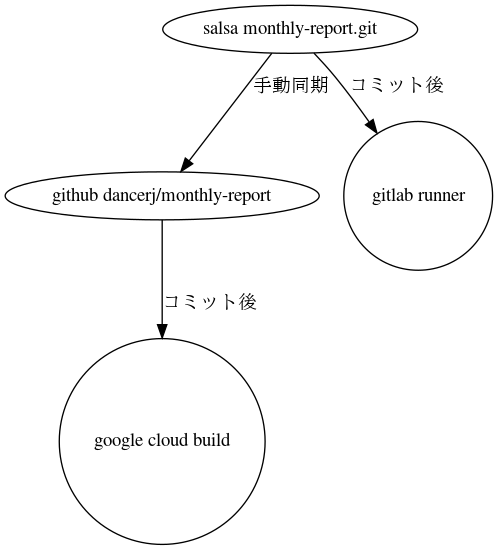
\includegraphics[keepaspectratio,width=0.5\hsize]{../2020/image202011/debci.png}
\end{center}
\caption{CIの流れ}
\label{fig:monthlyreport-ci-configuration}
\end{figure}

本当はsalsaのmasterにpushされる前にビルドのチェックを走らせたいのですが
できるのかな?

CIの設定ファイルが複数あるのも今後の課題です。

\begin{itemize}
 \item cloudbuild.yaml -- cloud buildで使っている。
 \item utils/docker/cloudbuild.yaml -- docker image 作成用
 \item .gitlab-ci.yml -- salsaの設定
 \item debian/control -- 2013年ころまで pbuilder ベースで走らせていたCI用、現在は何に利用しているのか?
\end{itemize}

最初はDebian環境にLaTeX環境のインストールとセットアップからするように設
定していたのですが、様子を見ている限りだとLaTeX関連のパッケージに何分も
かかっているようでした。Docker Imageをたまに更新するようにしてそれを利用
すればより高速になる気がしており、試しにDocker Imageを事前に作成するよう
にしたらCloud Buildの時間が13分くらいに短縮されました。

Docker Imageはとりあえず手元のraspberry pi 3 で定期的に更新するようにし
ています。



%for less page
%\printindex

\newpage

\begin{center}
本資料のライセンスについて
\end{center}

\begin{fontsize}{6}{6}

本資料はフリー・ソフトウェアです。あなたは、Free Software
Foundation が公表したGNU GENERAL PUBLIC LICENSEの "バージョン2"もしくはそれ以降
が定める条項に従って本プログラムを再頒布または変更することができ
ます。

本プログラムは有用とは思いますが、頒布にあたっては、市場性及び特
定目的適合性についての暗黙の保証を含めて、いかなる保証も行ないま
せん。詳細についてはGNU GENERAL PUBLIC LICENSE をお読みください。

\end{fontsize}

\begin{center}
ソースコードについて
\end{center}

本資料のソースコードは Git を使って\url{https://salsa.debian.org/tokyodebian-team/monthly-report.git}
からダウンロードできます。以下に方法を示します。

\begin{commandline}
$ sudo apt update
$ sudo apt install git
$ git clone https://salsa.debian.org/tokyodebian-team/monthly-report.git
\end{commandline}
%$

\begin{multicols}{2}
 \begin{fontsize}{6}{6}
 \begin{verbatim}
            GNU GENERAL PUBLIC LICENSE
               Version 2, June 1991

 Copyright (C) 1989, 1991 Free Software Foundation, Inc.
    51 Franklin St, Fifth Floor, Boston, MA  02110-1301  USA
 Everyone is permitted to copy and distribute verbatim copies
 of this license document, but changing it is not allowed.

                Preamble

  The licenses for most software are designed to take away your
freedom to share and change it.  By contrast, the GNU General Public
License is intended to guarantee your freedom to share and change free
software--to make sure the software is free for all its users.  This
General Public License applies to most of the Free Software
Foundation's software and to any other program whose authors commit to
using it.  (Some other Free Software Foundation software is covered by
the GNU Library General Public License instead.)  You can apply it to
your programs, too.

  When we speak of free software, we are referring to freedom, not
price.  Our General Public Licenses are designed to make sure that you
have the freedom to distribute copies of free software (and charge for
this service if you wish), that you receive source code or can get it
if you want it, that you can change the software or use pieces of it
in new free programs; and that you know you can do these things.

  To protect your rights, we need to make restrictions that forbid
anyone to deny you these rights or to ask you to surrender the rights.
These restrictions translate to certain responsibilities for you if you
distribute copies of the software, or if you modify it.

  For example, if you distribute copies of such a program, whether
gratis or for a fee, you must give the recipients all the rights that
you have.  You must make sure that they, too, receive or can get the
source code.  And you must show them these terms so they know their
rights.

  We protect your rights with two steps: (1) copyright the software, and
(2) offer you this license which gives you legal permission to copy,
distribute and/or modify the software.

  Also, for each author's protection and ours, we want to make certain
that everyone understands that there is no warranty for this free
software.  If the software is modified by someone else and passed on, we
want its recipients to know that what they have is not the original, so
that any problems introduced by others will not reflect on the original
authors' reputations.

  Finally, any free program is threatened constantly by software
patents.  We wish to avoid the danger that redistributors of a free
program will individually obtain patent licenses, in effect making the
program proprietary.  To prevent this, we have made it clear that any
patent must be licensed for everyone's free use or not licensed at all.

  The precise terms and conditions for copying, distribution and
modification follow.

            GNU GENERAL PUBLIC LICENSE
   TERMS AND CONDITIONS FOR COPYING, DISTRIBUTION AND MODIFICATION

  0. This License applies to any program or other work which contains
a notice placed by the copyright holder saying it may be distributed
under the terms of this General Public License.  The "Program", below,
refers to any such program or work, and a "work based on the Program"
means either the Program or any derivative work under copyright law:
that is to say, a work containing the Program or a portion of it,
either verbatim or with modifications and/or translated into another
language.  (Hereinafter, translation is included without limitation in
the term "modification".)  Each licensee is addressed as "you".

Activities other than copying, distribution and modification are not
covered by this License; they are outside its scope.  The act of
running the Program is not restricted, and the output from the Program
is covered only if its contents constitute a work based on the
Program (independent of having been made by running the Program).
Whether that is true depends on what the Program does.

  1. You may copy and distribute verbatim copies of the Program's
source code as you receive it, in any medium, provided that you
conspicuously and appropriately publish on each copy an appropriate
copyright notice and disclaimer of warranty; keep intact all the
notices that refer to this License and to the absence of any warranty;
and give any other recipients of the Program a copy of this License
along with the Program.

You may charge a fee for the physical act of transferring a copy, and
you may at your option offer warranty protection in exchange for a fee.

  2. You may modify your copy or copies of the Program or any portion
of it, thus forming a work based on the Program, and copy and
distribute such modifications or work under the terms of Section 1
above, provided that you also meet all of these conditions:

    a) You must cause the modified files to carry prominent notices
    stating that you changed the files and the date of any change.

    b) You must cause any work that you distribute or publish, that in
    whole or in part contains or is derived from the Program or any
    part thereof, to be licensed as a whole at no charge to all third
    parties under the terms of this License.

    c) If the modified program normally reads commands interactively
    when run, you must cause it, when started running for such
    interactive use in the most ordinary way, to print or display an
    announcement including an appropriate copyright notice and a
    notice that there is no warranty (or else, saying that you provide
    a warranty) and that users may redistribute the program under
    these conditions, and telling the user how to view a copy of this
    License.  (Exception: if the Program itself is interactive but
    does not normally print such an announcement, your work based on
    the Program is not required to print an announcement.)

These requirements apply to the modified work as a whole.  If
identifiable sections of that work are not derived from the Program,
and can be reasonably considered independent and separate works in
themselves, then this License, and its terms, do not apply to those
sections when you distribute them as separate works.  But when you
distribute the same sections as part of a whole which is a work based
on the Program, the distribution of the whole must be on the terms of
this License, whose permissions for other licensees extend to the
entire whole, and thus to each and every part regardless of who wrote it.

Thus, it is not the intent of this section to claim rights or contest
your rights to work written entirely by you; rather, the intent is to
exercise the right to control the distribution of derivative or
collective works based on the Program.

In addition, mere aggregation of another work not based on the Program
with the Program (or with a work based on the Program) on a volume of
a storage or distribution medium does not bring the other work under
the scope of this License.

  3. You may copy and distribute the Program (or a work based on it,
under Section 2) in object code or executable form under the terms of
Sections 1 and 2 above provided that you also do one of the following:

    a) Accompany it with the complete corresponding machine-readable
    source code, which must be distributed under the terms of Sections
    1 and 2 above on a medium customarily used for software interchange; or,

    b) Accompany it with a written offer, valid for at least three
    years, to give any third party, for a charge no more than your
    cost of physically performing source distribution, a complete
    machine-readable copy of the corresponding source code, to be
    distributed under the terms of Sections 1 and 2 above on a medium
    customarily used for software interchange; or,

    c) Accompany it with the information you received as to the offer
    to distribute corresponding source code.  (This alternative is
    allowed only for noncommercial distribution and only if you
    received the program in object code or executable form with such
    an offer, in accord with Subsection b above.)

The source code for a work means the preferred form of the work for
making modifications to it.  For an executable work, complete source
code means all the source code for all modules it contains, plus any
associated interface definition files, plus the scripts used to
control compilation and installation of the executable.  However, as a
special exception, the source code distributed need not include
anything that is normally distributed (in either source or binary
form) with the major components (compiler, kernel, and so on) of the
operating system on which the executable runs, unless that component
itself accompanies the executable.

If distribution of executable or object code is made by offering
access to copy from a designated place, then offering equivalent
access to copy the source code from the same place counts as
distribution of the source code, even though third parties are not
compelled to copy the source along with the object code.

  4. You may not copy, modify, sublicense, or distribute the Program
except as expressly provided under this License.  Any attempt
otherwise to copy, modify, sublicense or distribute the Program is
void, and will automatically terminate your rights under this License.
However, parties who have received copies, or rights, from you under
this License will not have their licenses terminated so long as such
parties remain in full compliance.

  5. You are not required to accept this License, since you have not
signed it.  However, nothing else grants you permission to modify or
distribute the Program or its derivative works.  These actions are
prohibited by law if you do not accept this License.  Therefore, by
modifying or distributing the Program (or any work based on the
Program), you indicate your acceptance of this License to do so, and
all its terms and conditions for copying, distributing or modifying
the Program or works based on it.

  6. Each time you redistribute the Program (or any work based on the
Program), the recipient automatically receives a license from the
original licensor to copy, distribute or modify the Program subject to
these terms and conditions.  You may not impose any further
restrictions on the recipients' exercise of the rights granted herein.
You are not responsible for enforcing compliance by third parties to
this License.

  7. If, as a consequence of a court judgment or allegation of patent
infringement or for any other reason (not limited to patent issues),
conditions are imposed on you (whether by court order, agreement or
otherwise) that contradict the conditions of this License, they do not
excuse you from the conditions of this License.  If you cannot
distribute so as to satisfy simultaneously your obligations under this
License and any other pertinent obligations, then as a consequence you
may not distribute the Program at all.  For example, if a patent
license would not permit royalty-free redistribution of the Program by
all those who receive copies directly or indirectly through you, then
the only way you could satisfy both it and this License would be to
refrain entirely from distribution of the Program.

If any portion of this section is held invalid or unenforceable under
any particular circumstance, the balance of the section is intended to
apply and the section as a whole is intended to apply in other
circumstances.

It is not the purpose of this section to induce you to infringe any
patents or other property right claims or to contest validity of any
such claims; this section has the sole purpose of protecting the
integrity of the free software distribution system, which is
implemented by public license practices.  Many people have made
generous contributions to the wide range of software distributed
through that system in reliance on consistent application of that
system; it is up to the author/donor to decide if he or she is willing
to distribute software through any other system and a licensee cannot
impose that choice.

This section is intended to make thoroughly clear what is believed to
be a consequence of the rest of this License.

  8. If the distribution and/or use of the Program is restricted in
certain countries either by patents or by copyrighted interfaces, the
original copyright holder who places the Program under this License
may add an explicit geographical distribution limitation excluding
those countries, so that distribution is permitted only in or among
countries not thus excluded.  In such case, this License incorporates
the limitation as if written in the body of this License.

  9. The Free Software Foundation may publish revised and/or new versions
of the General Public License from time to time.  Such new versions will
be similar in spirit to the present version, but may differ in detail to
address new problems or concerns.

Each version is given a distinguishing version number.  If the Program
specifies a version number of this License which applies to it and "any
later version", you have the option of following the terms and conditions
either of that version or of any later version published by the Free
Software Foundation.  If the Program does not specify a version number of
this License, you may choose any version ever published by the Free Software
Foundation.

  10. If you wish to incorporate parts of the Program into other free
programs whose distribution conditions are different, write to the author
to ask for permission.  For software which is copyrighted by the Free
Software Foundation, write to the Free Software Foundation; we sometimes
make exceptions for this.  Our decision will be guided by the two goals
of preserving the free status of all derivatives of our free software and
of promoting the sharing and reuse of software generally.

                NO WARRANTY

  11. BECAUSE THE PROGRAM IS LICENSED FREE OF CHARGE, THERE IS NO WARRANTY
FOR THE PROGRAM, TO THE EXTENT PERMITTED BY APPLICABLE LAW.  EXCEPT WHEN
OTHERWISE STATED IN WRITING THE COPYRIGHT HOLDERS AND/OR OTHER PARTIES
PROVIDE THE PROGRAM "AS IS" WITHOUT WARRANTY OF ANY KIND, EITHER EXPRESSED
OR IMPLIED, INCLUDING, BUT NOT LIMITED TO, THE IMPLIED WARRANTIES OF
MERCHANTABILITY AND FITNESS FOR A PARTICULAR PURPOSE.  THE ENTIRE RISK AS
TO THE QUALITY AND PERFORMANCE OF THE PROGRAM IS WITH YOU.  SHOULD THE
PROGRAM PROVE DEFECTIVE, YOU ASSUME THE COST OF ALL NECESSARY SERVICING,
REPAIR OR CORRECTION.

  12. IN NO EVENT UNLESS REQUIRED BY APPLICABLE LAW OR AGREED TO IN WRITING
WILL ANY COPYRIGHT HOLDER, OR ANY OTHER PARTY WHO MAY MODIFY AND/OR
REDISTRIBUTE THE PROGRAM AS PERMITTED ABOVE, BE LIABLE TO YOU FOR DAMAGES,
INCLUDING ANY GENERAL, SPECIAL, INCIDENTAL OR CONSEQUENTIAL DAMAGES ARISING
OUT OF THE USE OR INABILITY TO USE THE PROGRAM (INCLUDING BUT NOT LIMITED
TO LOSS OF DATA OR DATA BEING RENDERED INACCURATE OR LOSSES SUSTAINED BY
YOU OR THIRD PARTIES OR A FAILURE OF THE PROGRAM TO OPERATE WITH ANY OTHER
PROGRAMS), EVEN IF SUCH HOLDER OR OTHER PARTY HAS BEEN ADVISED OF THE
POSSIBILITY OF SUCH DAMAGES.

             END OF TERMS AND CONDITIONS

        How to Apply These Terms to Your New Programs

  If you develop a new program, and you want it to be of the greatest
possible use to the public, the best way to achieve this is to make it
free software which everyone can redistribute and change under these terms.

  To do so, attach the following notices to the program.  It is safest
to attach them to the start of each source file to most effectively
convey the exclusion of warranty; and each file should have at least
the "copyright" line and a pointer to where the full notice is found.

    <one line to give the program's name and a brief idea of what it does.>
    Copyright (C) <year>  <name of author>

    This program is free software; you can redistribute it and/or modify
    it under the terms of the GNU General Public License as published by
    the Free Software Foundation; either version 2 of the License, or
    (at your option) any later version.

    This program is distributed in the hope that it will be useful,
    but WITHOUT ANY WARRANTY; without even the implied warranty of
    MERCHANTABILITY or FITNESS FOR A PARTICULAR PURPOSE.  See the
    GNU General Public License for more details.

    You should have received a copy of the GNU General Public License
    along with this program; if not, write to the Free Software
    Foundation, Inc., 51 Franklin St, Fifth Floor, Boston, MA  02110-1301 USA


Also add information on how to contact you by electronic and paper mail.

If the program is interactive, make it output a short notice like this
when it starts in an interactive mode:

    Gnomovision version 69, Copyright (C) year  name of author
    Gnomovision comes with ABSOLUTELY NO WARRANTY; for details type `show w'.
    This is free software, and you are welcome to redistribute it
    under certain conditions; type `show c' for details.

The hypothetical commands `show w' and `show c' should show the appropriate
parts of the General Public License.  Of course, the commands you use may
be called something other than `show w' and `show c'; they could even be
mouse-clicks or menu items--whatever suits your program.

You should also get your employer (if you work as a programmer) or your
school, if any, to sign a "copyright disclaimer" for the program, if
necessary.  Here is a sample; alter the names:

  Yoyodyne, Inc., hereby disclaims all copyright interest in the program
  `Gnomovision' (which makes passes at compilers) written by James Hacker.

  <signature of Ty Coon>, 1 April 1989
  Ty Coon, President of Vice

This General Public License does not permit incorporating your program into
proprietary programs.  If your program is a subroutine library, you may
consider it more useful to permit linking proprietary applications with the
library.  If this is what you want to do, use the GNU Library General
Public License instead of this License.
 \end{verbatim}
 \end{fontsize}
\end{multicols}

\begin{center}
Debian オープンユーズロゴ ライセンス
\end{center}

\begin{multicols}{2}
 \begin{fontsize}{6}{6}
 \begin{verbatim}

Copyright (c) 1999 Software in the Public Interest
Permission is hereby granted, free of charge, to any person
obtaining a copy of this software and associated documentation
files (the "Software"), to deal in the Software without restriction,
including without limitation the rights to use, copy, modify, merge,
publish, distribute, sublicense, and/or sell copies of the Software,
and to permit persons to whom the Software is furnished to do so,
subject to the following conditions:

The above copyright notice and this permission notice shall be
included in all copies or substantial portions of the Software.

THE SOFTWARE IS PROVIDED "AS IS", WITHOUT WARRANTY OF ANY
KIND, EXPRESS OR IMPLIED, INCLUDING BUT NOT LIMITED TO THE
WARRANTIES OF MERCHANTABILITY, FITNESS FOR A PARTICULAR PURPOSE AND
NONINFRINGEMENT. IN NO EVENT SHALL THE AUTHORS OR COPYRIGHT HOLDERS
BE LIABLE FOR ANY CLAIM, DAMAGES OR OTHER LIABILITY, WHETHER IN
AN ACTION OF CONTRACT, TORT OR OTHERWISE, ARISING FROM, OUT OF OR
IN CONNECTION WITH THE SOFTWARE OR THE USE OR OTHER DEALINGS IN
THE SOFTWARE.
 \end{verbatim}
 \end{fontsize}
\end{multicols}

% 問題と回答が同じみひらきにならないようにする
%\cleartoevenpage
%-------------------------------------------------------------------------------
%\dancersection{Debian Trivia Quiz 問題回答}{}
%-------------------------------------------------------------------------------

 % Debian Trivia Quiz の問題回答です。
 % あなたは何問わかりましたか? \\
 %回答はdebianmeetingresume2014-fuyu.jqzというファイルに生成されるので、
 %それを手動でコピペして使う。
 % ここからコピペ
 % FIXME 問題が全部はいったらコピペすること
 %(progn (next-line 1)(insert-file "debianmeetingresume2013-fuyu.jqz") )
%\begin{enumerate}
%\end{enumerate}

% add page to even number
%\newpage
\cleartooddpage

\newpage
\thispagestyle{empty}\mbox{}
\newpage

\thispagestyle{empty}
{
\large
\begin{itembox}{\bf 『あんどきゅめんてっど でびあん』について}
本書は、東京および関西周辺で毎月行なわれている『東京エリア Debian 勉強会』および
『関西 Debian 勉強会』で
使用された資料・小ネタ・必殺技などを一冊にまとめたものです。
% FIXME: 範囲を修正すること。
収録範囲は2019/12〜2020/11まで
内容は無保証、つっこみなどがあれば勉強会にて。
\end{itembox}
}

\vspace*{16cm}
{\color{dancerlightblue}\rule{\hsize}{1mm}}
\vspace{2mm}

\includegraphics[width=2cm]{image200502/openlogo-nd.eps}
\noindent \Large \bf あんどきゅめんてっど でびあん 2021年冬号\\
\noindent \normalfont 2021年12月31日 \hspace{5mm}  初版第1刷発行\\
\noindent \normalfont 東京エリア Debian 勉強会/関西Debian 勉強会 (編集・印刷・発行)\\
{\color{dancerdarkblue}\rule{\hsize}{1mm}}

\end{document}
